\documentclass[a4paper,11pt,oneside]{book}

\usepackage{./layout/layout}	%Layout
\usepackage{float}



\newcommand{\docAuthor}{Luzian Raphael Aufdenblatten \& Julian Bischof }
\title{Magnetische Aufhängung}
\author{Luzian Raphael Aufdenblatten \& Julian Bischof}

\begin{document}

\pagestyle{AMZ}


%---------- | < Titlepage > | ----------
\thispagestyle{empty}
\begin{titlepage}
    \begin{center}
        \textbf{\huge{Hochschule Luzern}}\\
        \vspace{2mm}
        \large{Technik und Architektur}\\
        \vspace{5mm}
    \end{center}

    \vspace{0mm}

    \begin{center}
        
\includegraphics[trim=0cm 0cm 0cm 0cm,clip=true, width=0.7\linewidth]{./figure/cover_image.png}
        \addcontentsline{lof}{figure}{Cover image}\\
    \end{center} 

    %\vspace{2mm}

    \begin{center}
        \rule{\textwidth}{2pt}
    \end{center}

    \begin{center}
      \textbf{\huge{RT+L}}\\
        \vspace{2mm}
        \Large{\makeatletter \@title  \makeatother}\\
        \vspace{2mm}
        \large{Laborbericht}
    \end{center}

    \begin{center}
        \rule{\textwidth}{2pt}
    \end{center}

    \noindent\begin{minipage}{0.8\textwidth}
        \begin{flushleft}
            Authoren:\\
            \large{\makeatletter \@author \makeatother}\\
            \vspace{4mm}
        \end{flushleft}
    \end{minipage}

    \vspace{2mm}

    \begin{center}
        Luzern, \today 
    \end{center}

\end{titlepage}
\clearpage



%----- | < Introduction > | -----
%---------- | < Mainmatter > | ----------
\mainmatter		%activates arabic enumeration
%----- | < Section 1 > | -----
\chapter{Problemstellung}\label{chap:Problemstellung}
\section{Aufgabe 1}\label{sec:Aufgabe1}
	\subsection*{Blockschaltbild des geregelten Systems}\label{sub:block_regel}
	Das Blockschaltbild des geschlossenen Regelkreises ist in \autoref{dia:closed_loop} ersichtlich. Hierbei wird die Stecke wie auch das Stellglied  in $P$ zusammengefasst.
	$S$ bezeichnet dabei die Totzeit und den Fehler der durch den Laserdistanzmesser in das System eingeführt wird.


	\begin{figure}[h]
	\centering
	\begin{tikzpicture}[node distance=2cm]
		
      % Eingangsgröße
	\node (r) {};
	
	% Summenpunkt
	\node[circle, draw, right=of r] (sum) {};
	\node[below right=0.2pt and 0.1pt of sum] {$-$};
	\node[above left =2pt and 2pt of sum] {$+$};
	
	% Regler
	\node[draw, rectangle, minimum width=1cm, minimum height=1cm,,right=of sum] (controller) {C $\frac{h}{i}$};
	
	% Strecke
	\node[draw, rectangle,  minimum width=1cm, minimum height=1cm, right=of controller] (plant) {P};

	% Sensor
	\node[draw, rectangle,  minimum width=1cm, minimum height=1cm, below=0.5 of controller] (sensor) {S};
	
	% Ausgang
	\node[right=of plant] (y) {};
	
	% Verbindungslinien
	\draw[->] (r) -- (sum) node[midway, above]  {$x_{ref} (t) $};
	\draw[->] (sum) -- (controller) node[midway, above] {$x_{\text{err}}$};
	\draw[->] (controller) -- (plant) node[midway, above] {$i(t)$};
	\draw[->] (plant) -- (y)  node[midway, above]  {$x(t)$};
	
	% Rückführung: von Linie abzweigen und unten herum zurück
	\coordinate (tap) at ($(plant)!0.5!(y)$); % Punkt auf der Linie zwischen plant und y
	\coordinate (feedback) at ($(sum)+(0,-2)$); % Punkt unterhalb des Summenpunkts
	
	\draw[->] (tap) |- (sensor) -| (sum);
		
	\end{tikzpicture}
	\caption{Geschlossener Regelkreis}
	\label{dia:closed_loop}
\end{figure}

	
\section{Aufgabe 2}\label{sec:Aufgabe2}
	\subsection*{Blockschaltbild des geregelten Systems mit Vorsteuerung}\label{sub:block_regel_FF}
	Das Blockschaltbild aus \autoref{sec:Aufgabe1} wird in \autoref{dia:closed_loop_FF} um eine Vorsteuerung $FF$ erweitert.


	\begin{figure}[h]
	\centering
	\begin{tikzpicture}[node distance=2cm]
		
      % Eingangsgröße
	\node (r) {};
	
	% Summenpunkt
	\node[circle, draw, right=of r] (sum) {};
	\node[below right=0.2pt and 0.2pt of sum] {$-$};
	\node[below left =-5pt and 0.2pt of sum] {$+$};

	% Summenpunkt2
	\node[circle, draw, right=of controller] (sum2) {};
	\node[above right =0.2pt and -5pt of sum2] {$+$};
	\node[below left =-5pt and 0.2pt of sum2] {$+$};
	
	% Regler
	\node[draw, rectangle, minimum width=1cm, minimum height=1cm, right=of sum] (controller) {C $\frac{h}{i}$};
	
	% Strecke
	\node[draw, rectangle,  minimum width=1cm, minimum height=1cm, right=of sum2] (plant) {P};

	% Sensor
	\node[draw, rectangle,  minimum width=1cm, minimum height=1cm, below=0.5 of controller] (sensor) {S};

	% Vorsteuerung
	\node[draw, rectangle, minimum width=1cm, minimum height=1cm, above=0.5 of controller] (prescaler) {FF$\frac{h}{i}$};


	% Ausgang
	\node[right=of plant] (y) {};
	
	% Verbindungslinien
	\draw[->] (r) -- (sum) node[midway, above]  {$x_{ref} (t) $};
	\draw[->] (sum) -- (controller) node[midway, above] {$x_{\text{err}}$};
	\draw[->] (controller) -- (sum2) node[midway, above] {$i_C(t)$};
	\draw[->] (sum2) -- (plant) node[midway, above] {$i(t)$};
	\draw[->] (plant) -- (y)  node[midway, above]  {$x(t)$};
	
	% Rückführung: von Linie abzweigen und unten herum zurück
	\coordinate (tap) at ($(plant)!0.5!(y)$); % Punkt auf der Linie zwischen plant und y
	\coordinate (feedback) at ($(sum)+(0,-2)$); % Punkt unterhalb des Summenpunkts
	\coordinate (feedforward) at ($(sum2)+(0,1)$); % Punkt unterhalb des Summenpunkts
	\coordinate (tap_pre) at ($(sum)+(-0.5,0)$); % Punkt vor dem Summenpunkt
	
	\draw[->] (tap) |- (sensor) -| (sum);

	\draw[->] (tap_pre) |-  (prescaler) -| (feedforward) node[midway, above]{$i_{FF}(t)$} -- (sum2) ;
		
	\end{tikzpicture}
	\caption{Geschlossener Regelkreis erweitert mit einer Vorsteuerung}
	\label{dia:closed_loop_FF}
\end{figure}


\newcommand{\laplace}{%
  \tikz[baseline={(base)}, inner sep=0pt, outer sep=0pt]{
    % Solid and hollow dots as nodes
    \node[circle, fill, inner sep=1.5pt] (solid) at (0,0) {};
    \node[draw, circle, inner sep=1.5pt] (hollow) at (0,.5) {};
    % Connecting line
    \draw (solid) -- (hollow);
    % Baseline anchor
    \coordinate (base) at (0,0);
  }
}

\chapter{Modellierung}\label{chap:Modellierung}
\section{Aufgabe 3}\label{sec:Aufgabe3}
	\subsection*{Bewegungsdifferentialgleichung}\label{sub:diffeq}
	Aus der gegebenen Bewegungsdifferentialgleichung und der, mittels eines Polynoms dritten Grades approximierten, statischen Kennlinie $i_o(x) = a_i + b_ix +c_ix^2 + d_ix^3$ ergibt sich für die Bewegungsdifferentialgleichung \ref{eq:bewegungsgleichung}. 
	
	\begin{align}\label{eq:bewegungsgleichung}
		\ddot{x} &= g - g \cdot \frac{i^2}{i_0^2(x)} \nonumber\\
		\ddot{x} &= g - g \cdot \frac{i^2}{(a_i + b_ix +c_ix^2 + d_ix^3)^2}
	\end{align} 

\section{Aufgabe 4}\label{sec:Aufgabe4}
	\subsection*{Linearisierung}\label{sub:diffeq_lin}
	Zur Linearisierung der Bewegungsdifferentialgleichung wird folgende Struktur der linearisierten Differentialgleichung eingesetzt:

	\begin{align}\label{eq:lin_eq} 
		\Delta\ddot{x} &= k_x\Delta x + k_i\Delta i + k_s \Delta F_s
	\end{align} 

	Die Faktoren $k_x$, $k_i$ und $k_s$ werden aus \autoref{eq:bewegungsgleichung} in einem Arbeitspunkt $x_o$ und $\bar{i}$ bestimmt. Dazu wird \autoref{eq:bewegungsgleichung} jeweils nach $\delta x$, $\delta i$ und $\delta F_s$ abgeleitet. Da für den Versuch die Störkraft $F_s = 0$ angenommen wird, muss $k_s$ nocht ermittelt werden. 


	\begin{align} \label{eq:kx}
		k_x &= \left. \frac{\delta}{\delta x}  \left( g-g\frac{i^2}{(a_i+b_ix+c_ix^2+d_ix^3)^2} \right) \right|_{x_0, \bar{i}} \nonumber \\
			&= \left. \frac{\delta}{\delta x} \frac{-gi^2}{(a_i+b_ix+c_ix^2+d_ix^3)^2} \right|_{x_0,\bar{i}}  \nonumber \\
			&= \frac{2g\bar{i}^2(3d_ix_0^2 + 2c_ix_0+b)}{(d_ix_0^3+c_ix_0^2+b_ix_0+a)^3} 
	\end{align} 

	\begin{align} \label{eq:ki}
		k_i &= \left. \frac{\delta}{\delta i}  \left( g-g\frac{i^2}{(a_i+b_ix+c_ix^2+d_ix^3)^2} \right) \right|_{x_0, \bar{i}} \nonumber \\
			&= \left. \frac{\delta}{\delta i} \frac{-gi^2}{(a_i+b_ix+c_ix^2+d_ix^3)^2} \right|_{x_0,\bar{i}}  \nonumber \\
			&= \frac{-2g\bar{i}}{(a_i + b_ix_0 +c_ix_0^2 + d_ix_0^3)^2}
	\end{align} 

	Werden nun \autoref{eq:kx} und \ref{eq:ki} in \autoref{eq:lin_eq} eingesetzt ergibt sich:

	\begin{align}\label{eq:lin_eq_k} 
		\Delta\ddot{x} &= \frac{2g\bar{i}^2(3d_ix_0^2 + 2c_ix_0+b)}{(d_ix_0^3+c_ix_0^2+b_ix_0+a)^3}  \cdot \Delta x + \frac{-2g\bar{i}}{(a_i + b_ix_0 +c_ix_0^2 + d_ix_0^3)^2} \cdot \Delta i 
	\end{align} 

\section{Aufgabe 5}\label{sec:Aufgabe5}
	\subsection*{Übertragungsfunktion $G_{\mathrm{Strecke}}$ }\label{sub:transfer_Gstrecke}
	Um die Übertragungsfunktion der Prozesstrecke $G_{\mathrm{Strecke}}$ zu finden, kann erneut \autoref{eq:lin_eq} bzw. \autoref{eq:lin_eq_k} genutzt werden.


	\begin{align}\label{eq:G_strecke} 
		\Delta \ddot{x} &= k_x \Delta x + k_i \Delta i \nonumber\\
		\laplace \nonumber \\
		s^2 \Delta X &= k_x \Delta X + k_i \Delta I  \notag  \\
		G_{\mathrm{Strecke}}(s) &= \frac{\Delta X}{\Delta I} = \frac{k_i}{s^2-kx} \nonumber\\
		G_{\mathrm{Strecke}}(s) &= \frac{\frac{-2g\bar{i}}{(a_i + b_ix_0 +c_ix_0^2 + d_ix_0^3)^2}}{s^2-\frac{2g\bar{i}^2(3d_ix_0^2 + 2c_ix_0+b)}{(d_ix_0^3+c_ix_0^2+b_ix_0+a)^3}}
	\end{align}

\newpage 

\section{Aufgabe 6}\label{sec:Aufgabe6}
	\subsection*{Statische Vorsteuerung}\label{sub:statisch_ff}
	Der Einsatz einer statischen Vorsteuerung besteht darin, dass kein Regelfehler $e(t)$ nötig ist und somit nicht auf die Rückmeldung des Sensors gewartet werden muss. Die Regelung wird schneller.


\section{Aufgabe 7}\label{sec:Aufgabe6}
	\subsection*{Statische Vorsteuerung}\label{sub:statisch_ff}
	Die statischen Vorsteuerungen $V_{\mathrm{L}}$ und 	$V_{\mathrm{NL}}$ ergeben sich aus $G_{\mathrm{Strecke}}^{-1}(s)$ wie folgt:
	
	\begin{align}\label{eq:VL} 
		V_{\mathrm{L}} &= \left. G_{\mathrm{Strecke}}^{-1}(s) \right |_{s = 0} = \left. \frac{s^2-kx}{k_i} \right |_{s = 0}  \nonumber\\
		V_{\mathrm{L}} &= \frac{-kx}{k_i}
	\end{align} 
	\begin{align}\label{eq:VL} 
		V_{\mathrm{NL}} &= \left. G_{\mathrm{Strecke}}^{-1}(s) \right |_{s = 0} = \left. \frac{s^2-kx}{k_i} \right |_{s = 0}  \nonumber\\
		V_{\mathrm{NL}} &= |d + cx_0^1 + bx_0^2 + ax_0^3|
	\end{align} 

\section{Aufgabe 8}\label{sec:Aufgabe8}
	\subsection*{Übertragungsfunktion $G_{\mathrm{Stell}}$ }\label{sub:transfer_Gstell}
	Mit der gegebenen Differentialgleichung des Stellglieds $u = Ri +L\frac{\mathrm{d}i}{\mathrm{d}t}$ kann die Übertragungsfunktion des Stellglieds $G_{\mathrm{Stell}}$ wie folgt gefunden werden:

	\begin{align}\label{eq:G_stell} 
		u &= Ri +L\frac{\mathrm{d}i}{\mathrm{d}t} \nonumber \\
		\laplace \nonumber \\
		U &= RI + sLI \nonumber \\
		G_{\mathrm{Stell}}(s) &= \frac{I}{U} = \frac{1}{R+Ls} = \frac{1}{1+\frac{L}{R}s}
	\end{align}
\newpage
\section{Aufgaben 9 und 10}\label{sec:Aufgabe9_10}
\subsection*{Nachstellzeit $T_{\mathrm{i}}$ des Stellgliedreglers und Übertragungsfunktion des Stellglieds}\label{sub:transfer_Ti_Cstell}

Der Regler des Stellglieds besteht aus einem PI-Regler mit Übertragungsfunktion $C_{\mathrm{Stell}} = K_{PS} \left(1+\frac{1}{s+T_i} \right)$. Damit ergibt sich für das geregelte Stellglied: 
	\begin{align}\label{eq:G_stell_closed} 
		G_{\mathrm{StellClosed}} &= \frac{L_{\mathrm{Stell}}}{1 + L_{\mathrm{Stell}}} = \frac{C_{ \mathrm{Stell}}G_{\mathrm{Stell}} }{1 +  C_{\mathrm{Stell}}G_{\mathrm{Stell}}}	
	\end{align}

	Hierbei zeigt sich, dass mit $T_{s} = \frac{L}{R} = T_{i}$ ein PT-1 erreicht werden kann:
	\begin{align}\label{eq:L_stell} 
		L_{\mathrm{Stell}}  &= K_{PS} \left(1+\frac{1}{s+T_i} \right) \cdot \frac{K_{S}}{1 + T_{S}s} \nonumber \\
							&= K_{PS} K_{S} \cdot \frac{1 + T_{S}}{T_{S}\left( 1 + T_{S} \right)} = \frac{K_{PS} K_{S} }{T_{S}}
	\end{align}

	Wird nun  \autoref{eq:L_stell} in \autoref{eq:G_stell_closed} eingesetzt ergibt sich die Übertragungsfunktion:
	\begin{align}\label{eq:G_stell_closed2} 
		G_{\mathrm{StellClosed}} &= \frac{K_{PS} K_{S}}{T_{s}s + K_{PS} K_{\mathrm{S}}}
	\end{align}



\section{Aufgabe 11}\label{sec:Aufgabe11}
	\subsection*{Übertragungsfunktion $G_{\mathrm{Sensor}}$ }\label{sub:transfer_Gsensor}
	Wir wissen, dass der sensor eine Totzeit $T_{t\mathrm{Sensor}}$ von $2.5 \si{\milli\second}$ aufweist. Somit kann seine Übertragungsfunktion $G_{\mathrm{Sensor}}$ mittels eines PT-1 Glieds beschrieben werden:

	\begin{align}\label{eq:G_sens} 
	G_{\mathrm{Sensor}} &= \frac{\Delta X_{m}}{\Delta X} = \frac{1}{1 + T_{t\mathrm{Sensor}}s}
	\end{align}












\chapter{Reglerentwruf und Versuchsdurchführung}\label{chap:versuch}
	\subsection*{Ermittlung der Kennlinie}
	Zur Ermittlung der Kennlinie wurde an 4 Punkten der Strom gemessen, bei welchem $F_g = F_{mag}$ galt und somit der Ball nach oben gezogen wurde.

	\begin{table}[!h]
			\renewcommand{\arraystretch}{1.2}
			\centering
			\caption{Tabelle zur Ermittlung der Kennlinie}
			\begin{zebratabular}{m{3cm} m{3cm}}
				\rowcolor{gray}
				\textbf{$x [m]$}	& \textbf{$i [A]$}		    \\
				$0.035$				& $0.398$  \\ 
				$0.040$				& $0.505$  \\
				$0.045$				& $0.6369$ \\
				$0.050$				& $0.8964$ \\
			\end{zebratabular}
			\renewcommand{\arraystretch}{1.0}
			\label{tab:kenn_strom}
		\end{table}
		Die Polynomfaktoren werden ebenfalls aus diesen Messungen bestimmt:
			\begin{figure}[H]
				\centering
				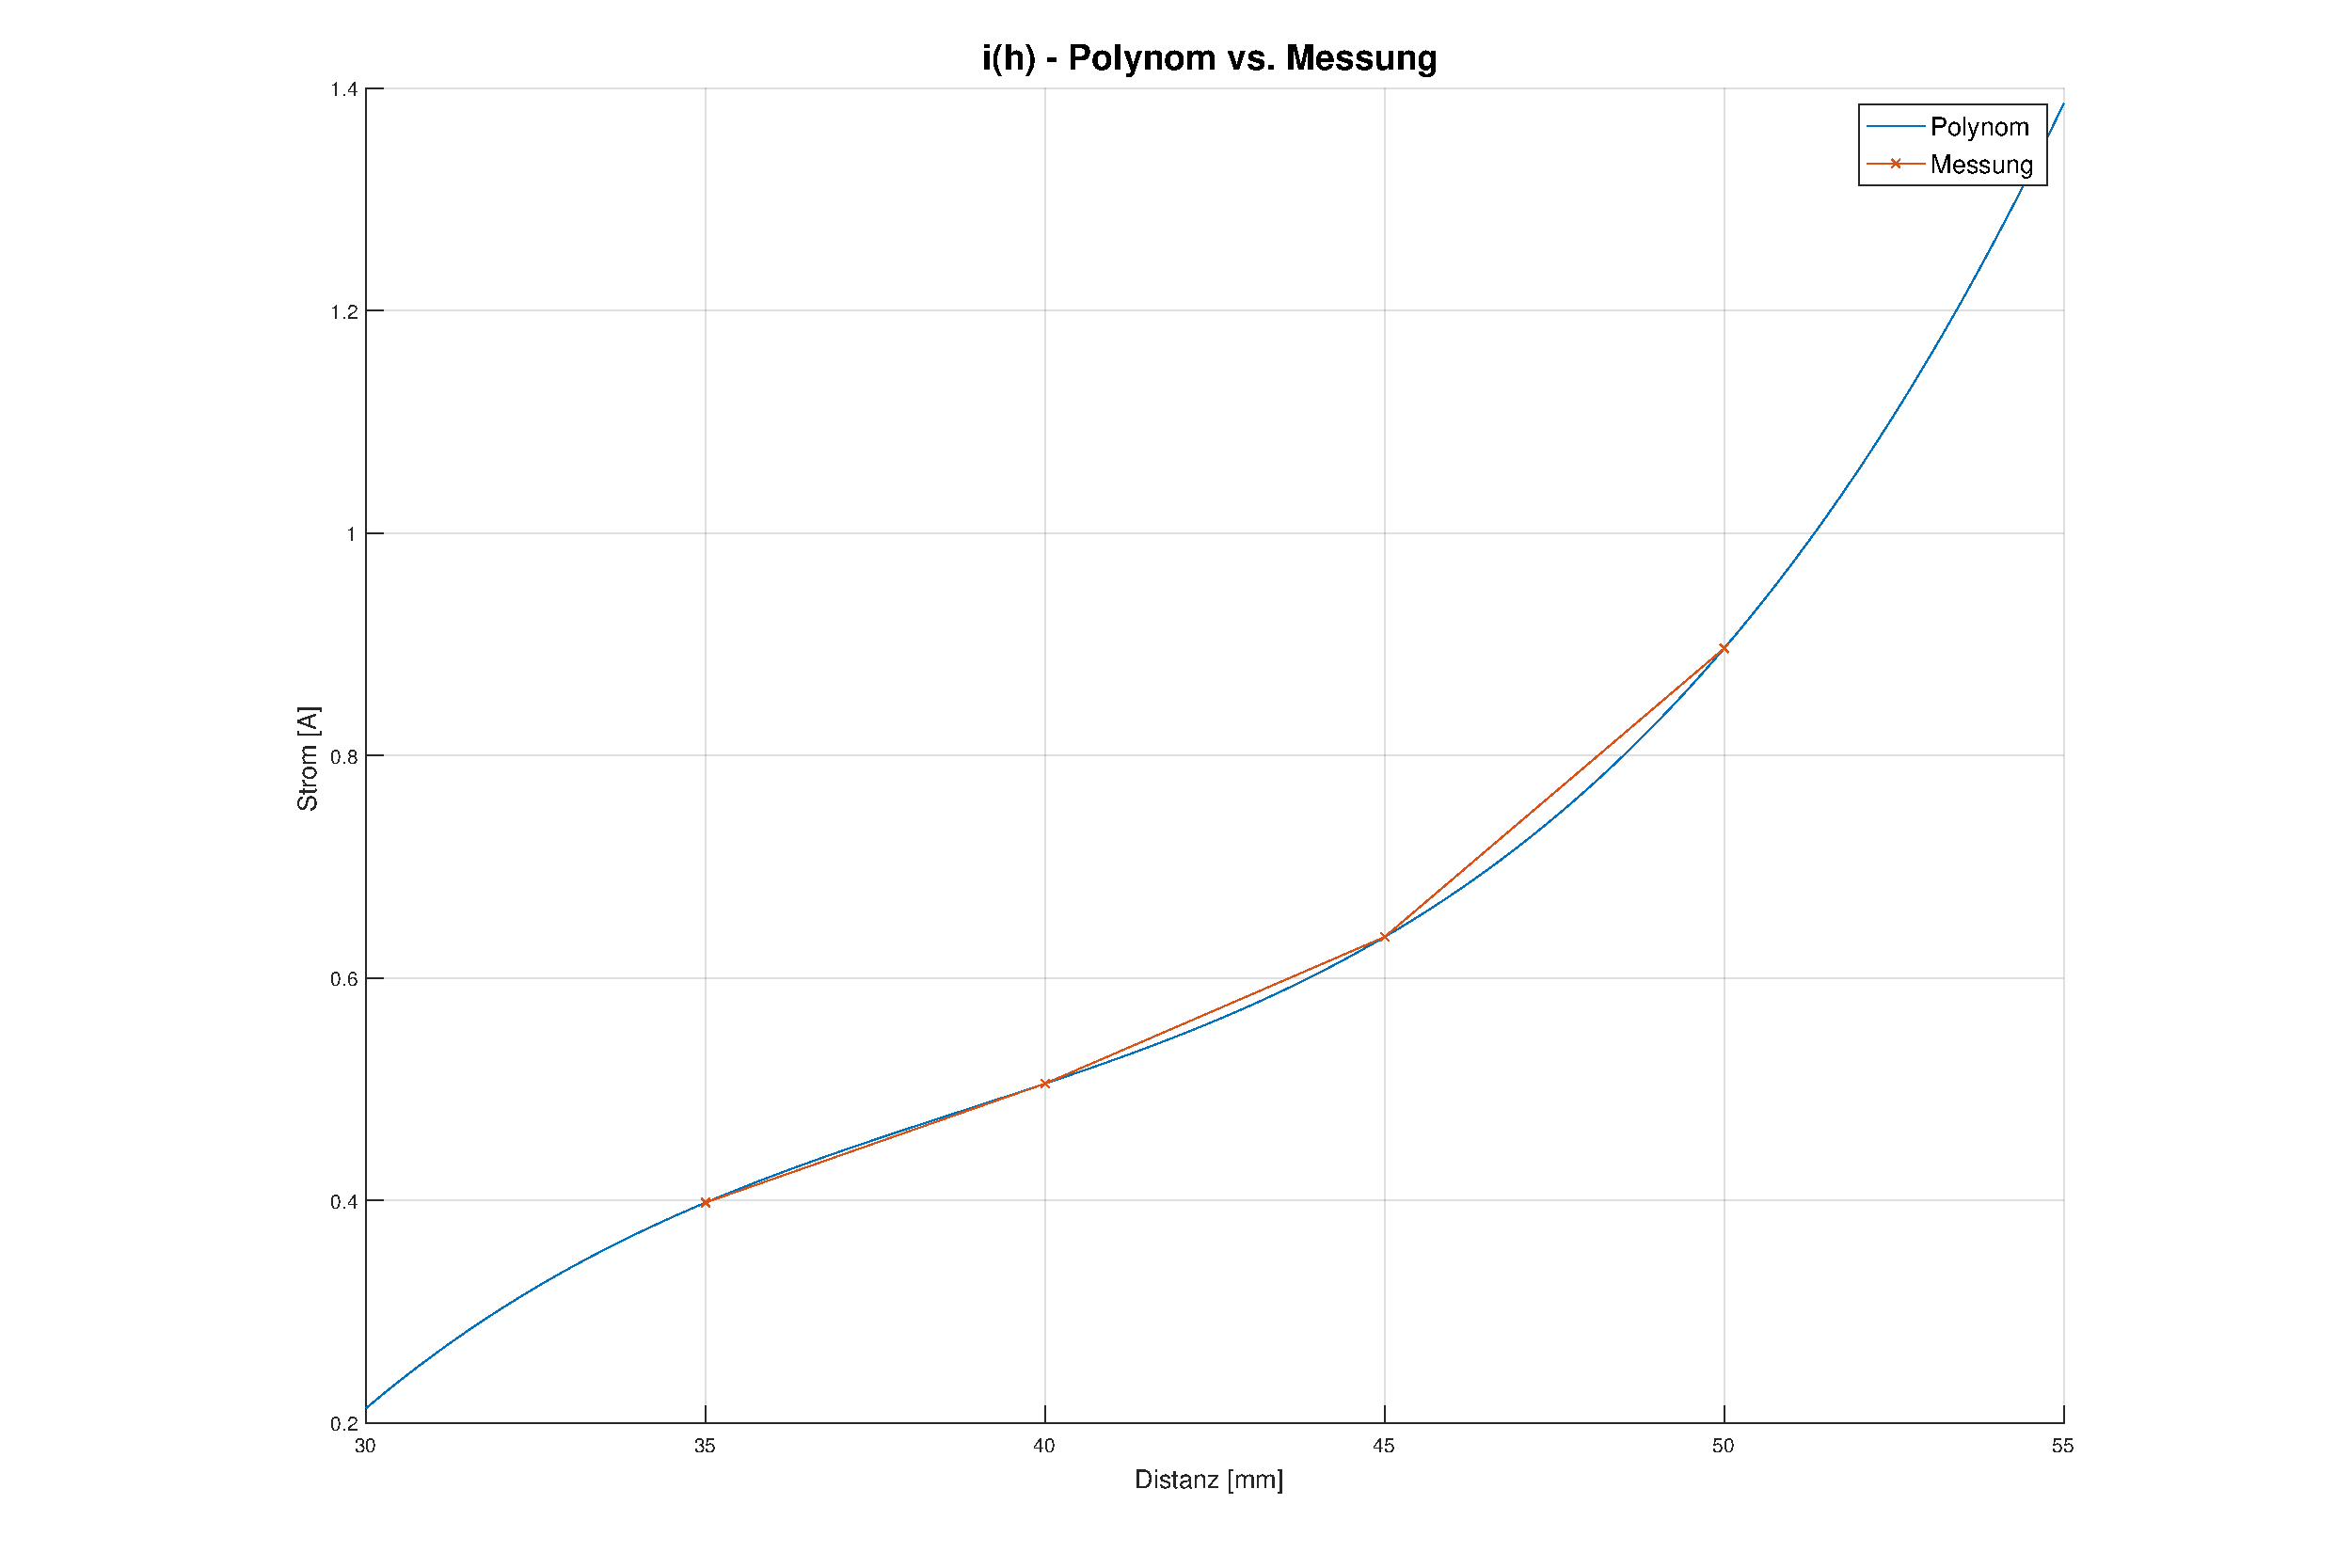
\includegraphics[width=.9\textwidth]{./figure/abstand_polyfit.pdf}
				\caption{Gemessene Punkte überlagert mit gefundenem Polynom}
				\label{fig:poly}
			\end{figure}
\newpage	
\section{Aufgabe 12}\label{sec:Aufgabe12}
	\subsection*{Vorzeichen der Reglerverstärkung}
	Das Vorzeichen von $K_{p}$ ist positiv.

\section{Aufgaben 13, 14 und 15}\label{sec:Aufgabe13_14}
	\subsection*{Wurzelortskurve des PD-Reglers}
	Durch Untersuchen der Wurzelortskurve (rlocus \autoref{fig:rlocusPD})  kann mit der Wahl von $T_d = \frac{1}{\sqrt{k_x}}$ erkannt werden, dass eine Verstärkung $K_p \geq 40$ nötig ist, um alle Pole in die negative Halbebene zu bewegen.
	\begin{figure}[H]
				\centering
				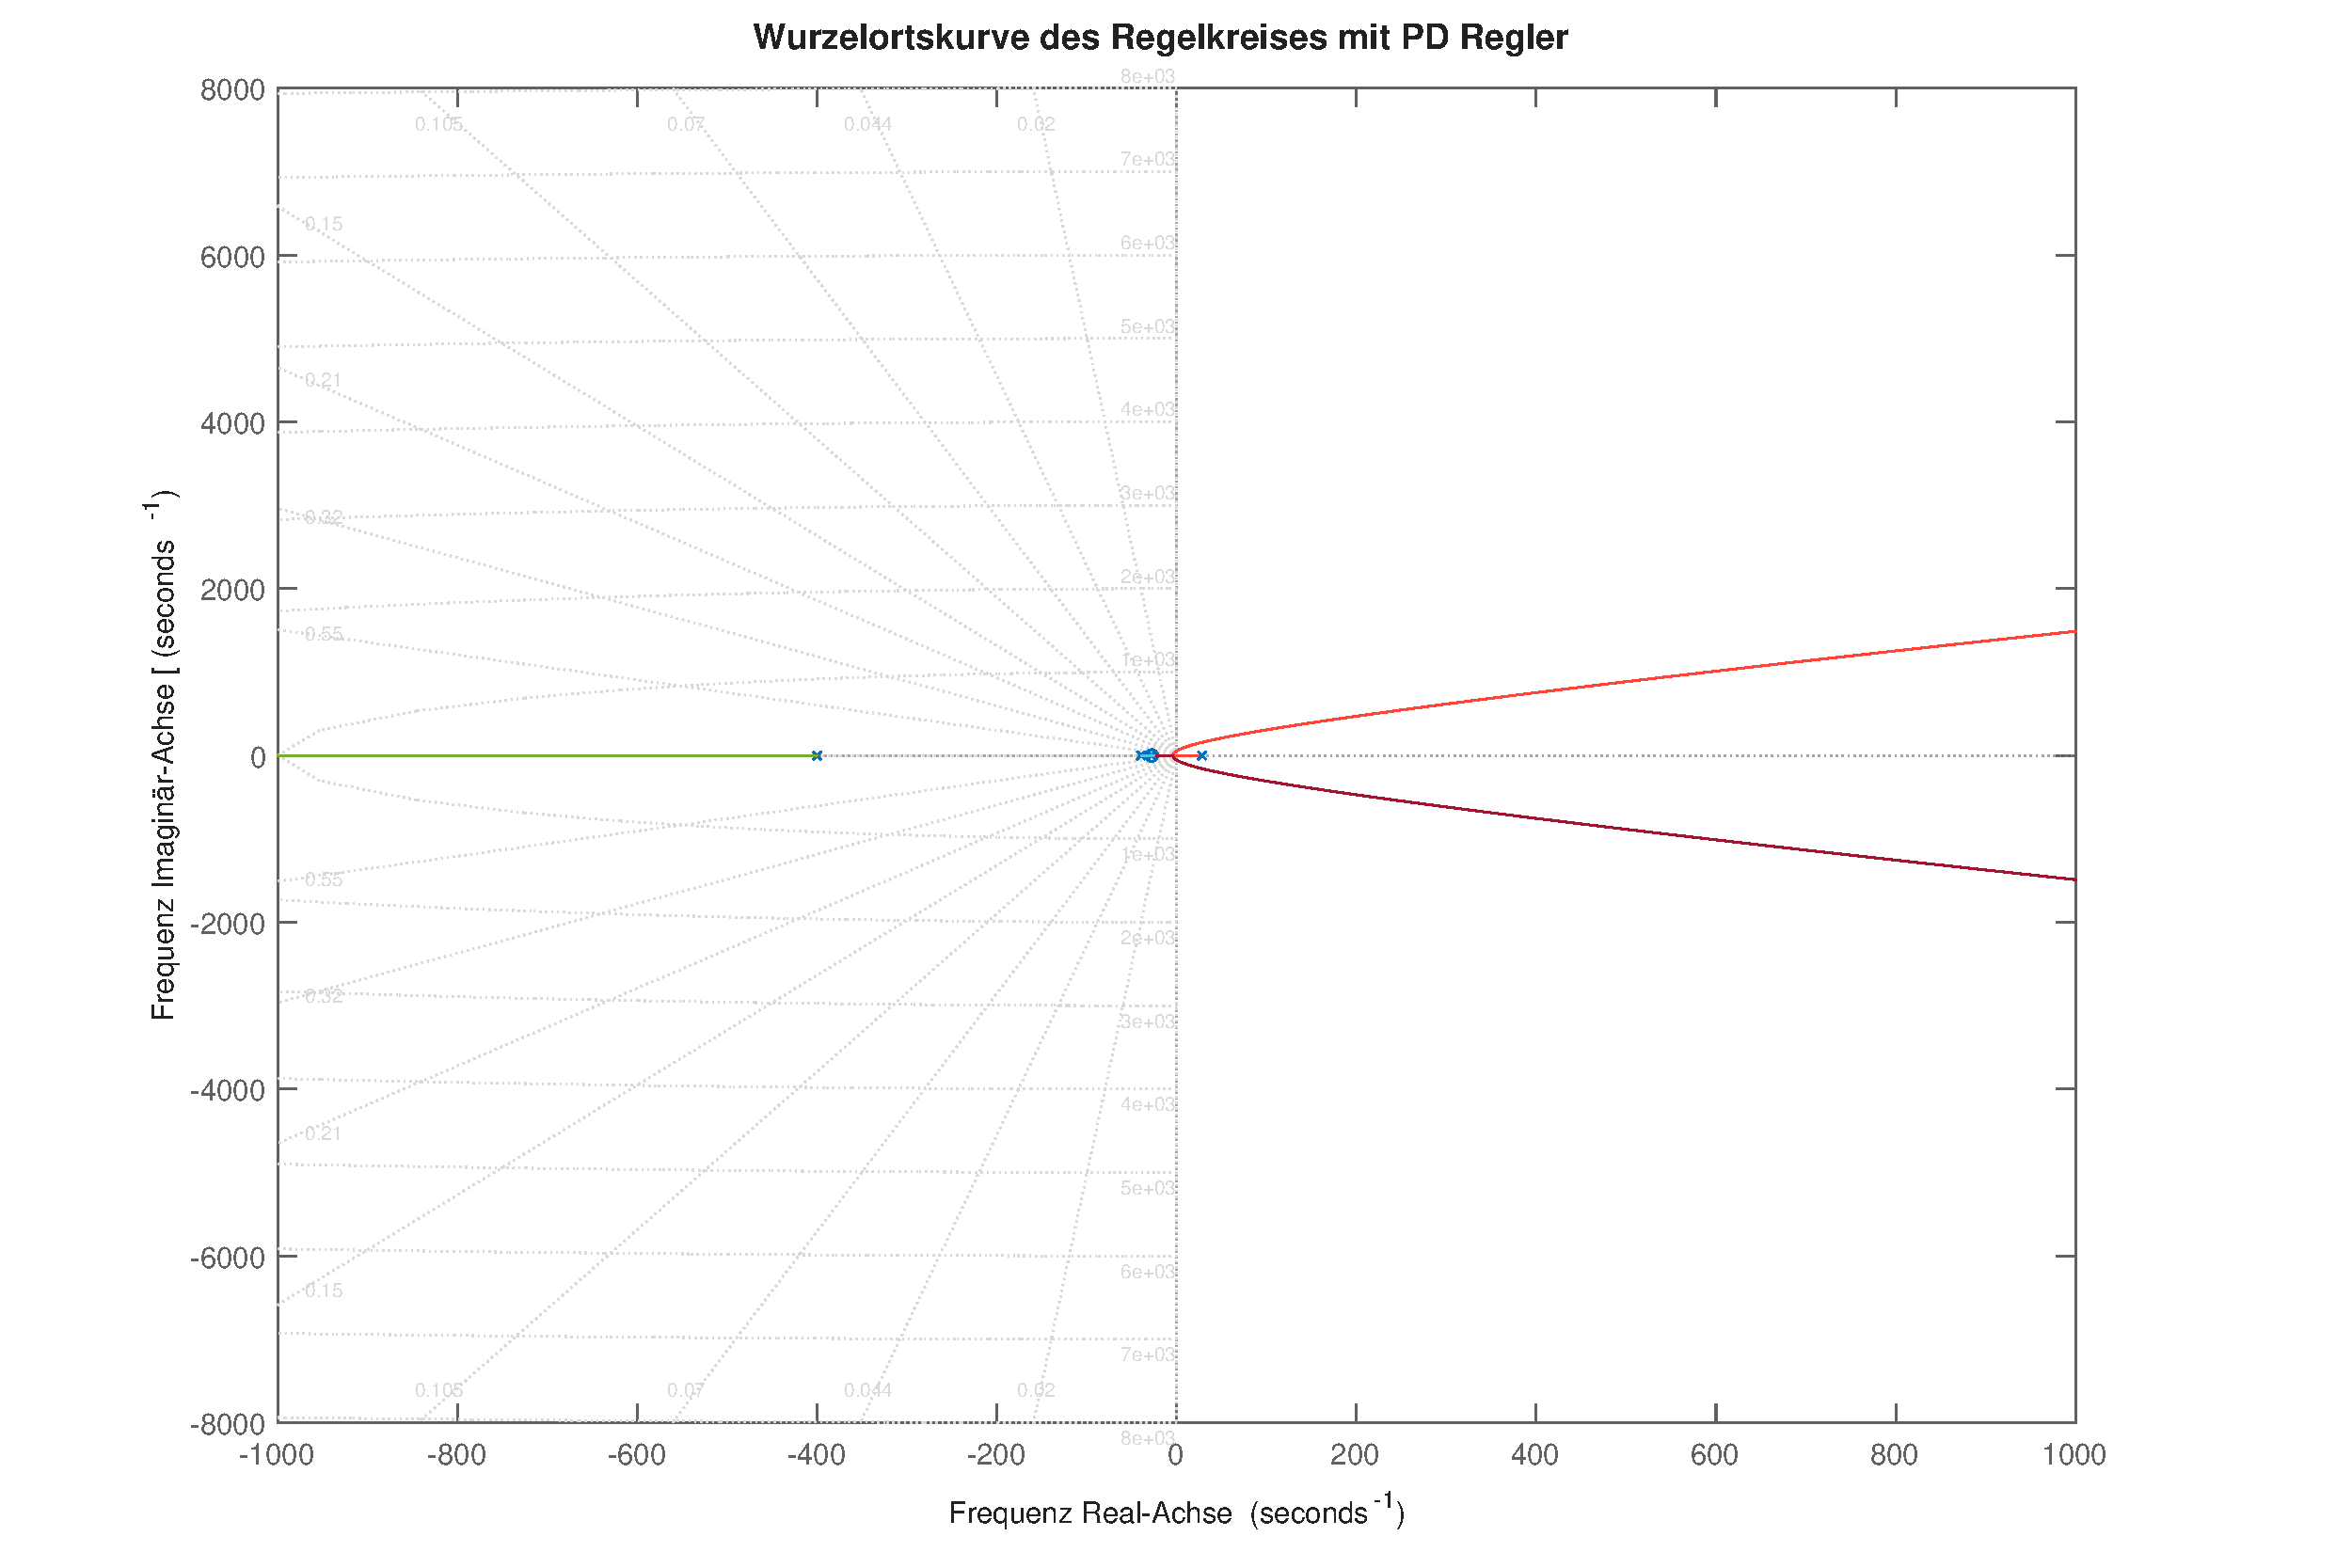
\includegraphics[width=.9\textwidth]{./figure/rlocus_pd_untuned.pdf}
				\caption{Wurzelortskurve des Prozesses mit PD-Regler}
				\label{fig:rlocusPD}
			\end{figure}


			Somit ergibt sich ein PD Regler $C_{PD} = K_p \cdot \left(  1 + T_d \frac{s}{\frac{N}{T_d}s + 1} \right)$ mit $K_p=40, T_d = \frac{1}{\sqrt{k_x}}$ und $N=100$.
			\newpage
			In \autoref{fig:polePD} ist erkenntlich, dass alle Pole in der linken (negativen) Halbebene liegen.

			\begin{figure}[H]
				\centering
				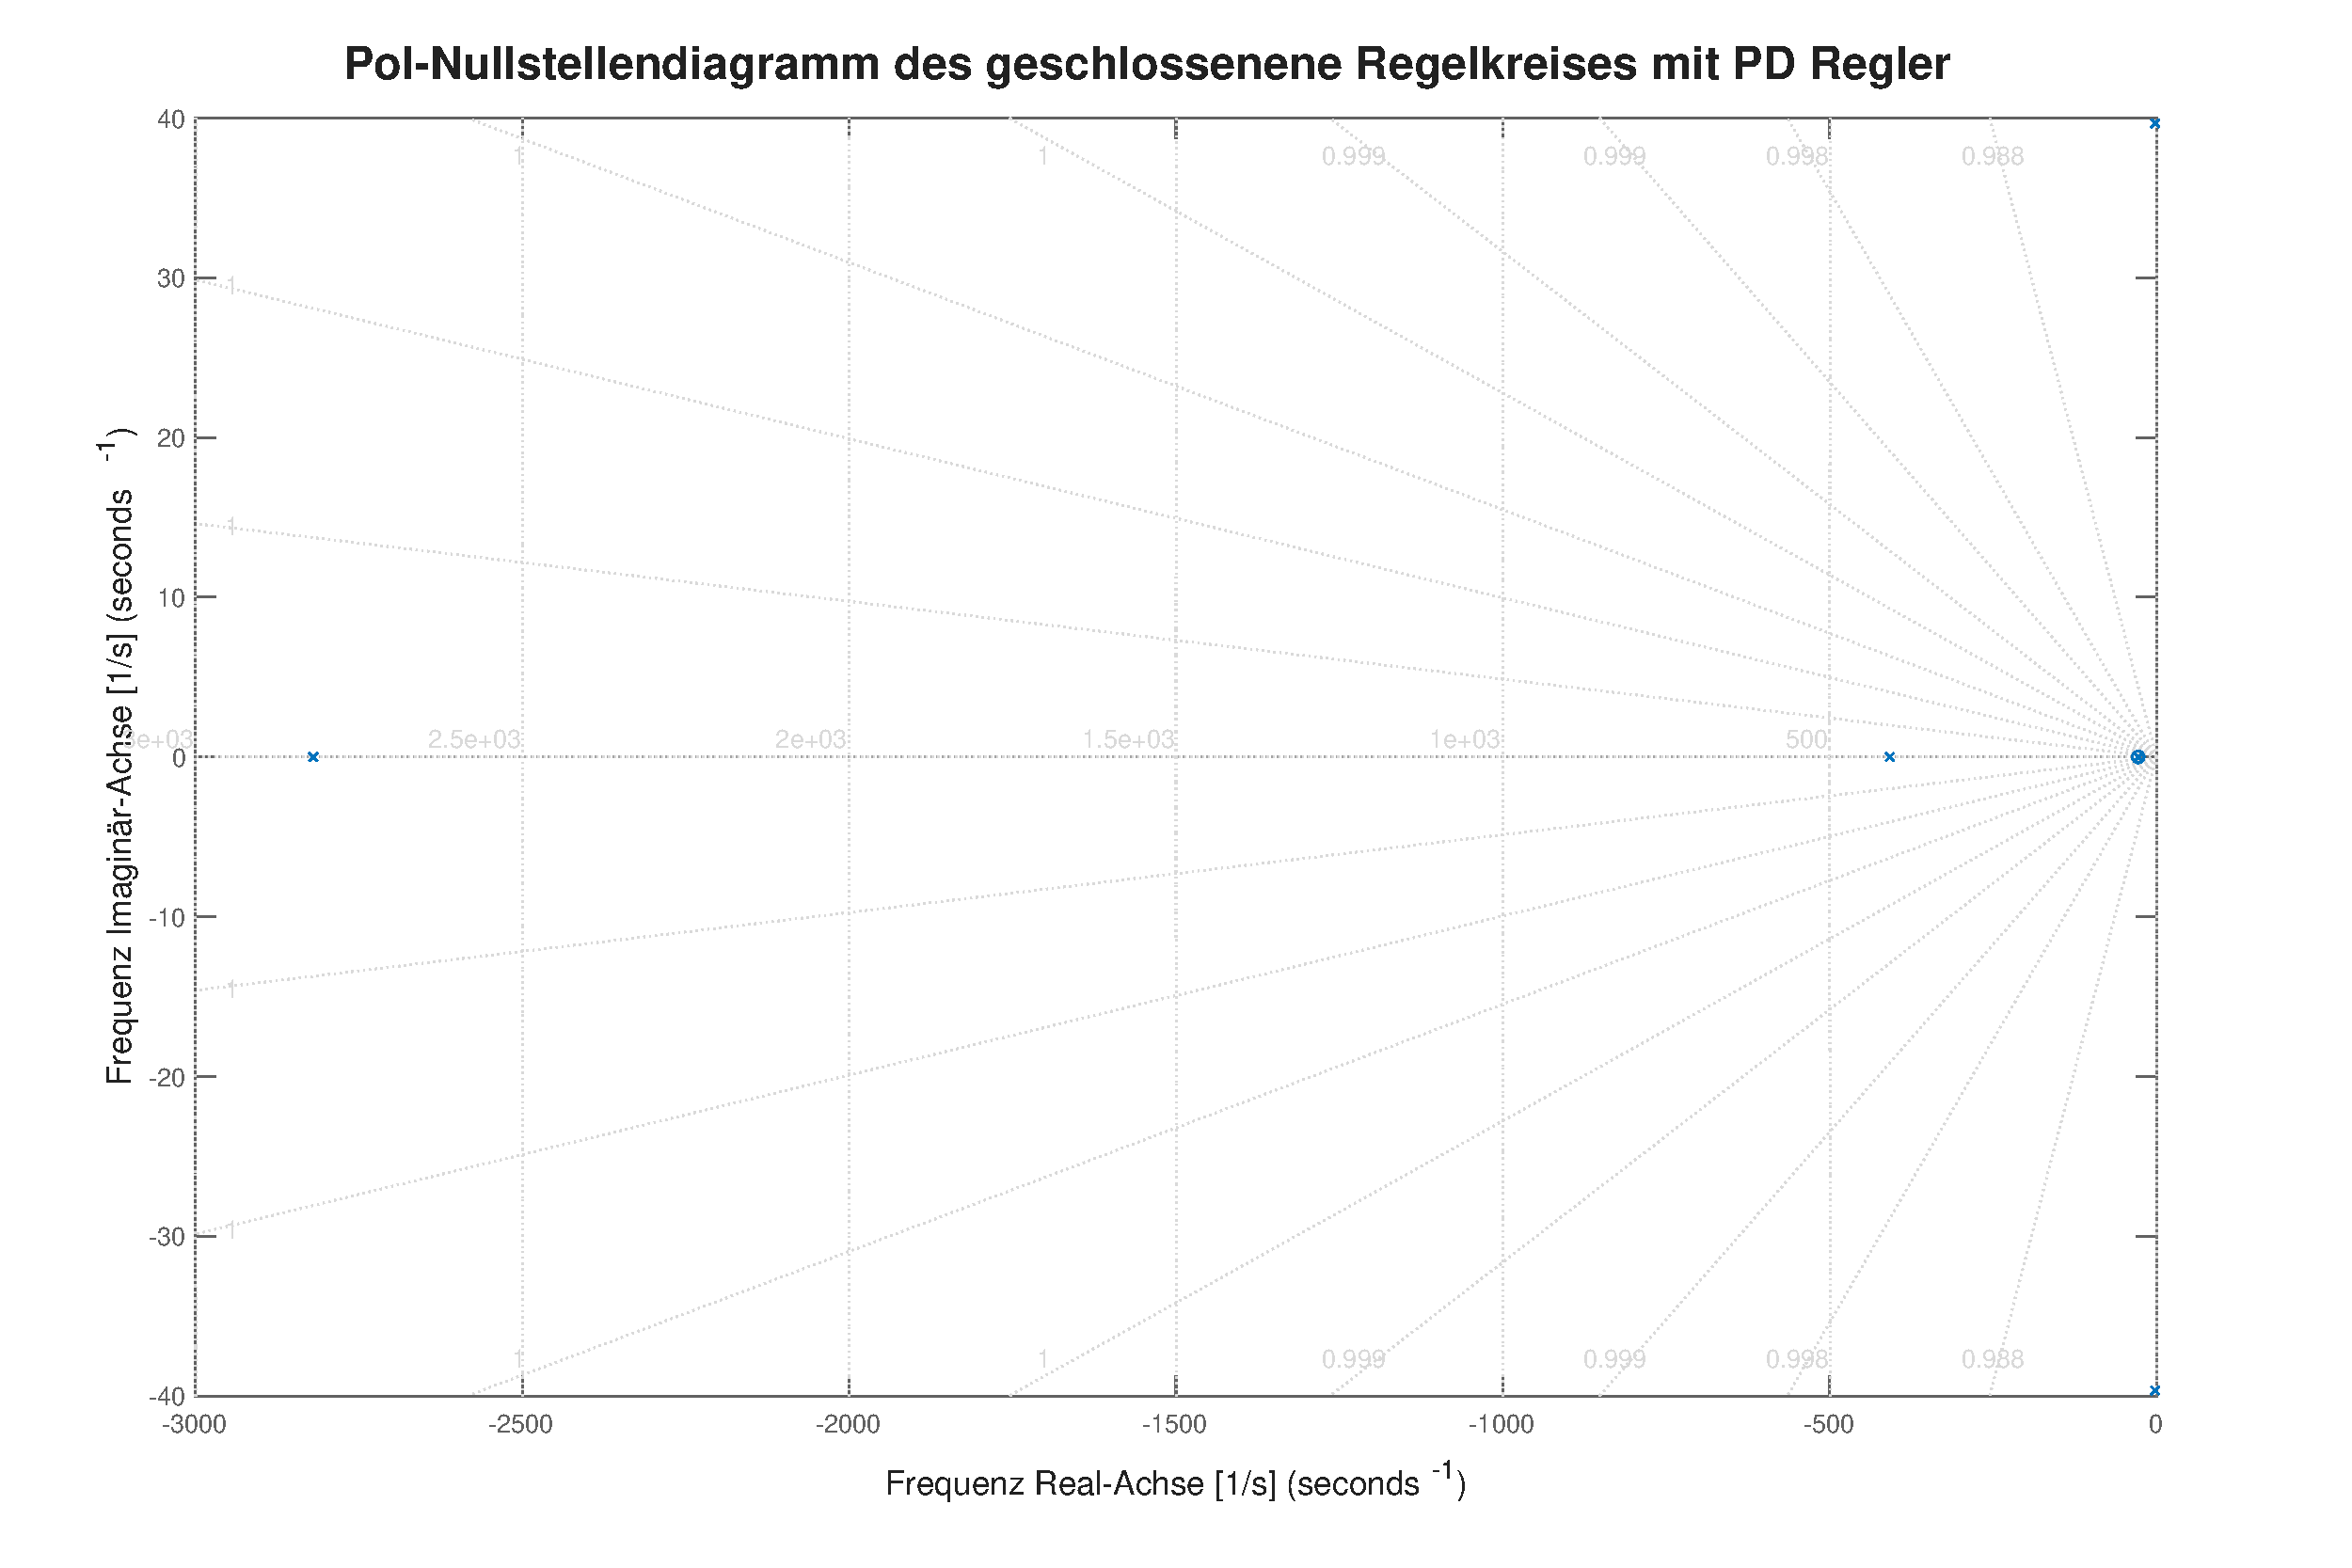
\includegraphics[width=.9\textwidth]{./figure/polemap_pd_untuned.pdf}
				\caption{Pole des Prozesses mit PD-Regler}
				\label{fig:polePD}
			\end{figure}
\newpage
	\subsection*{Erweiterung zum PID-Regler}
	Mit der gegebenen Vorschrift von $T_d < 0.25 T_i$ wurde zusammen mit Untersuchung der Wurzelortskurve ein Wert von $T_i = \frac{T_d}{T_i} + 0.1$ ermittelt.



	\begin{figure}[H]
				\centering
				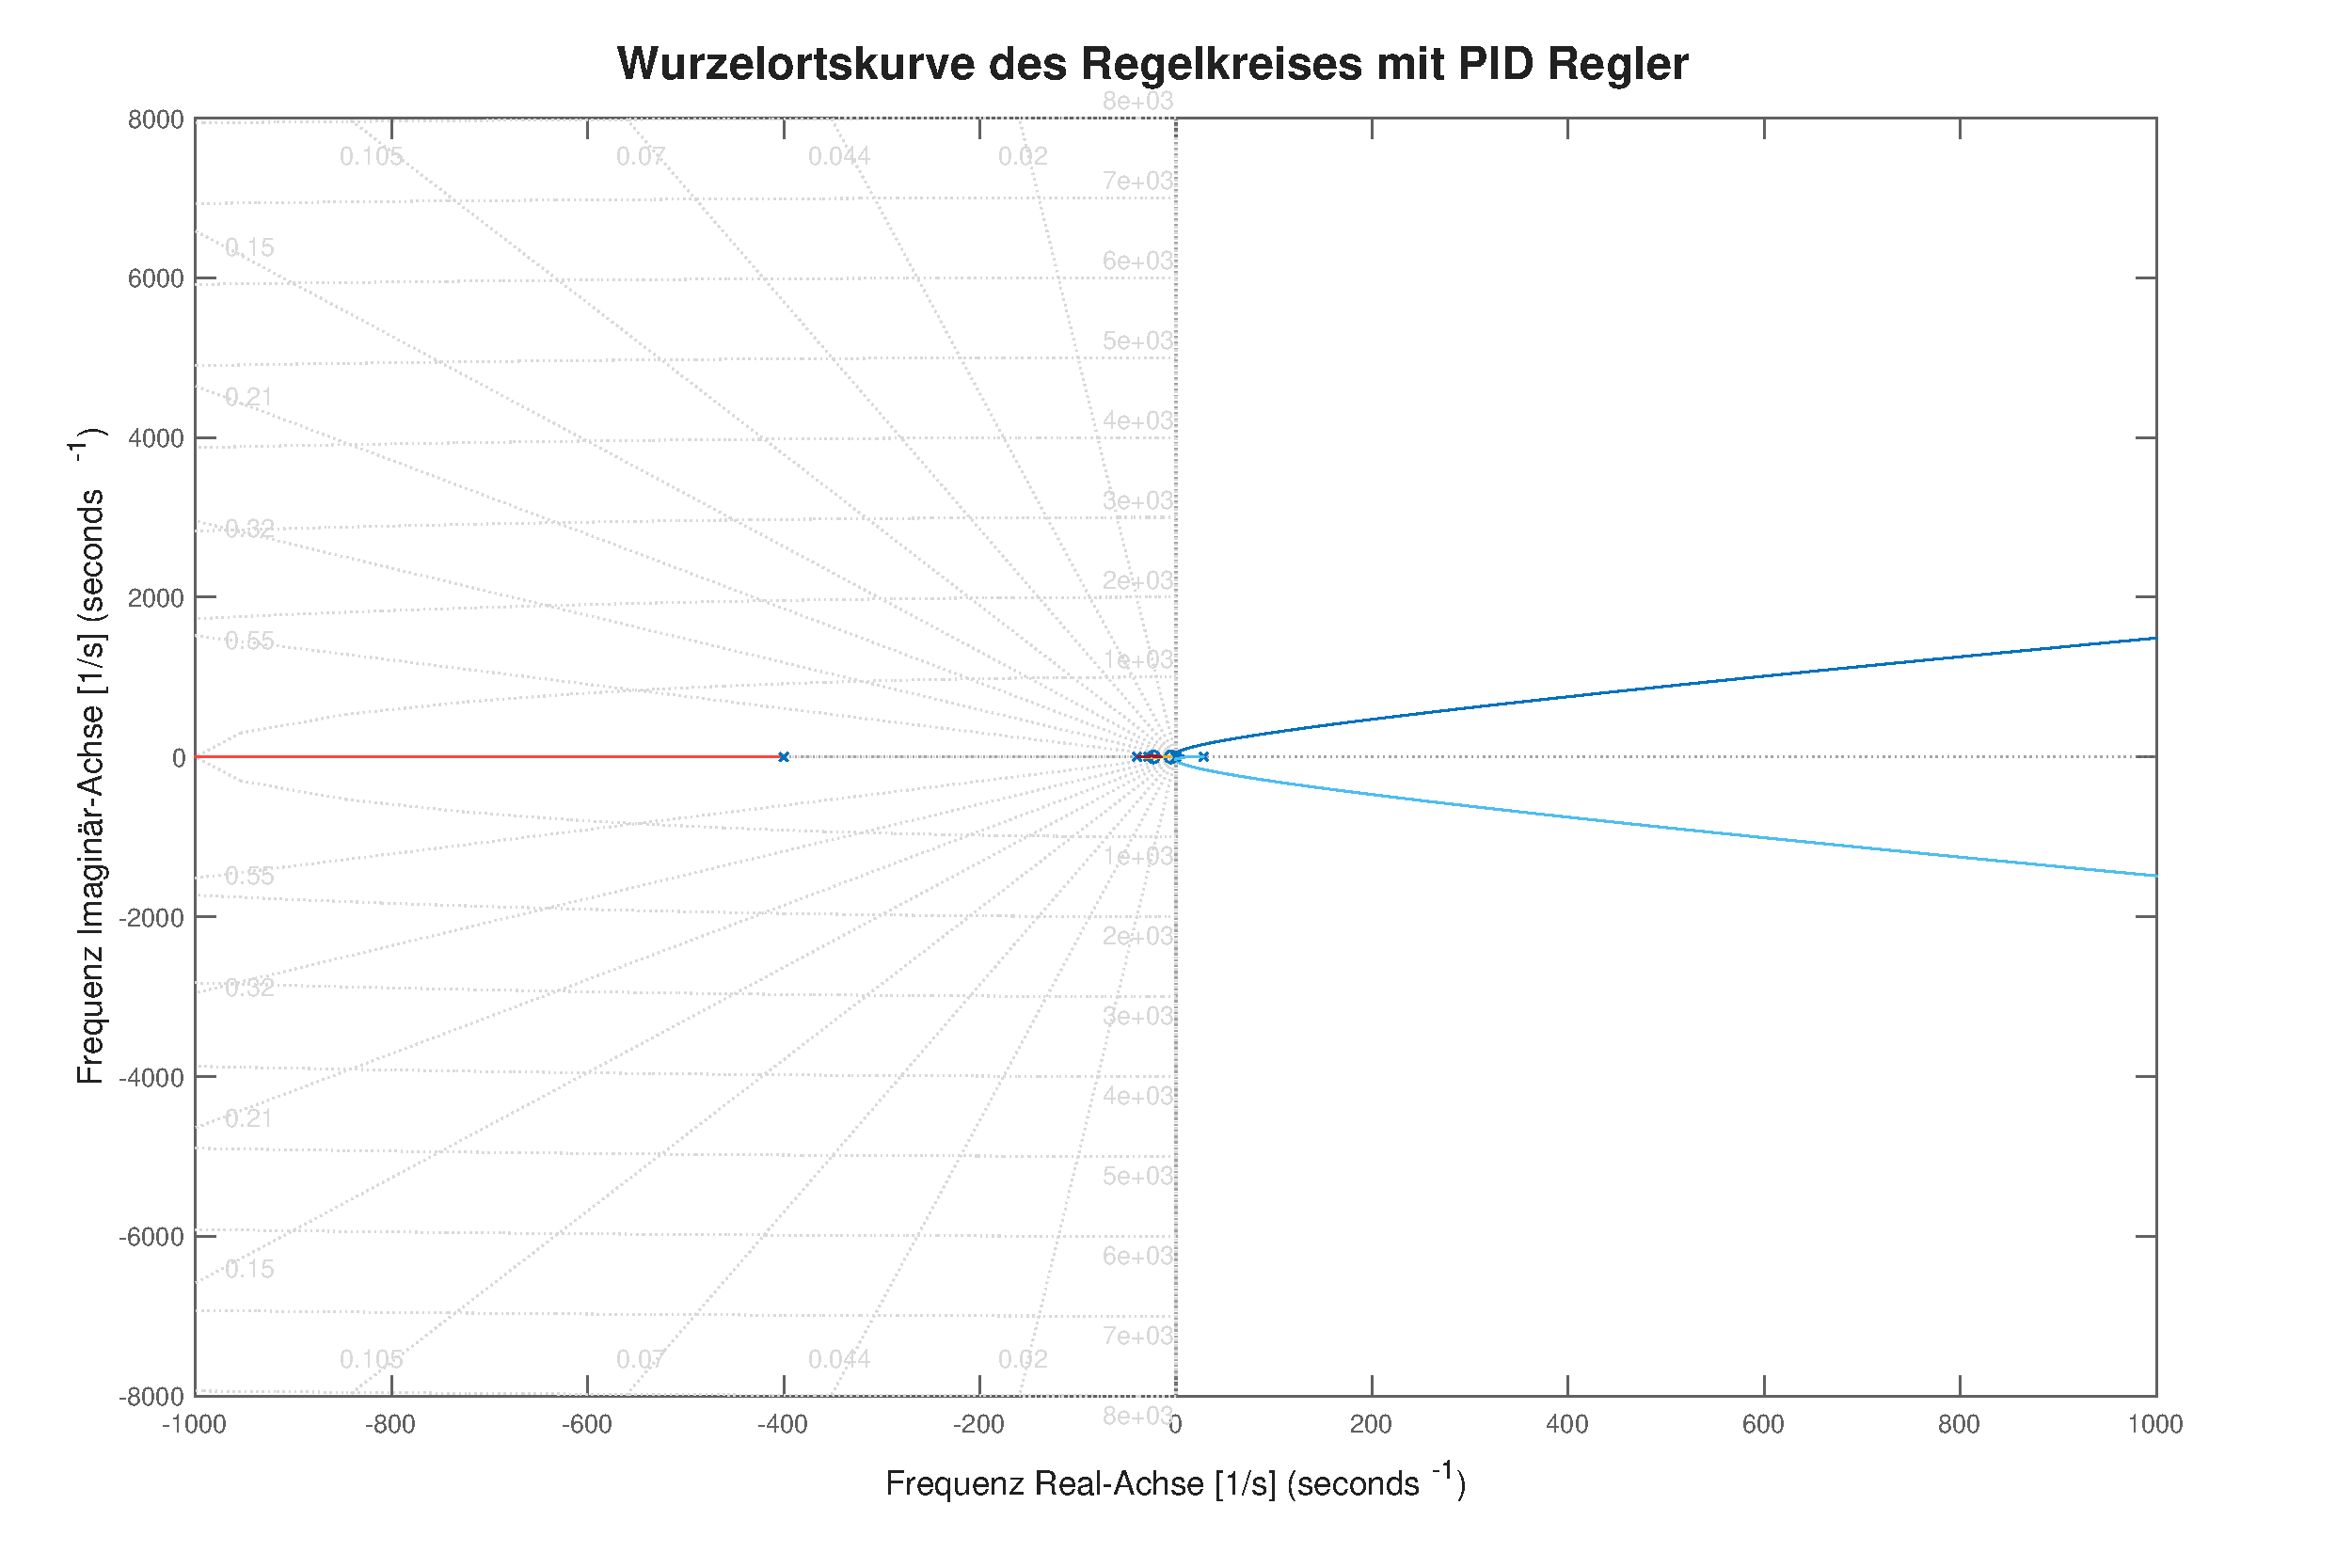
\includegraphics[width=.9\textwidth]{./figure/rlocus_pid_untuned.pdf}
				\caption{Wurzelortskurve des Prozesses mit PD-Regler}
				\label{fig:rlocusPID}
			\end{figure}


			Somit ergibt sich ein PID Regler $C_{PD} = K_p \cdot \left(  1 +\frac{1}{T_i}\cdot \frac{1}{s} + T_d \frac{s}{\frac{N}{T_d}s + 1} \right)$ mit $K_p=40, T_d = \frac{1}{\sqrt{k_x}}$ und $N=100$.
			\newpage
			In \autoref{fig:polePID} ist erkenntlich, dass alle Pole in der linken (negativen) Halbebene liegen.

			\begin{figure}[H]
				\centering
				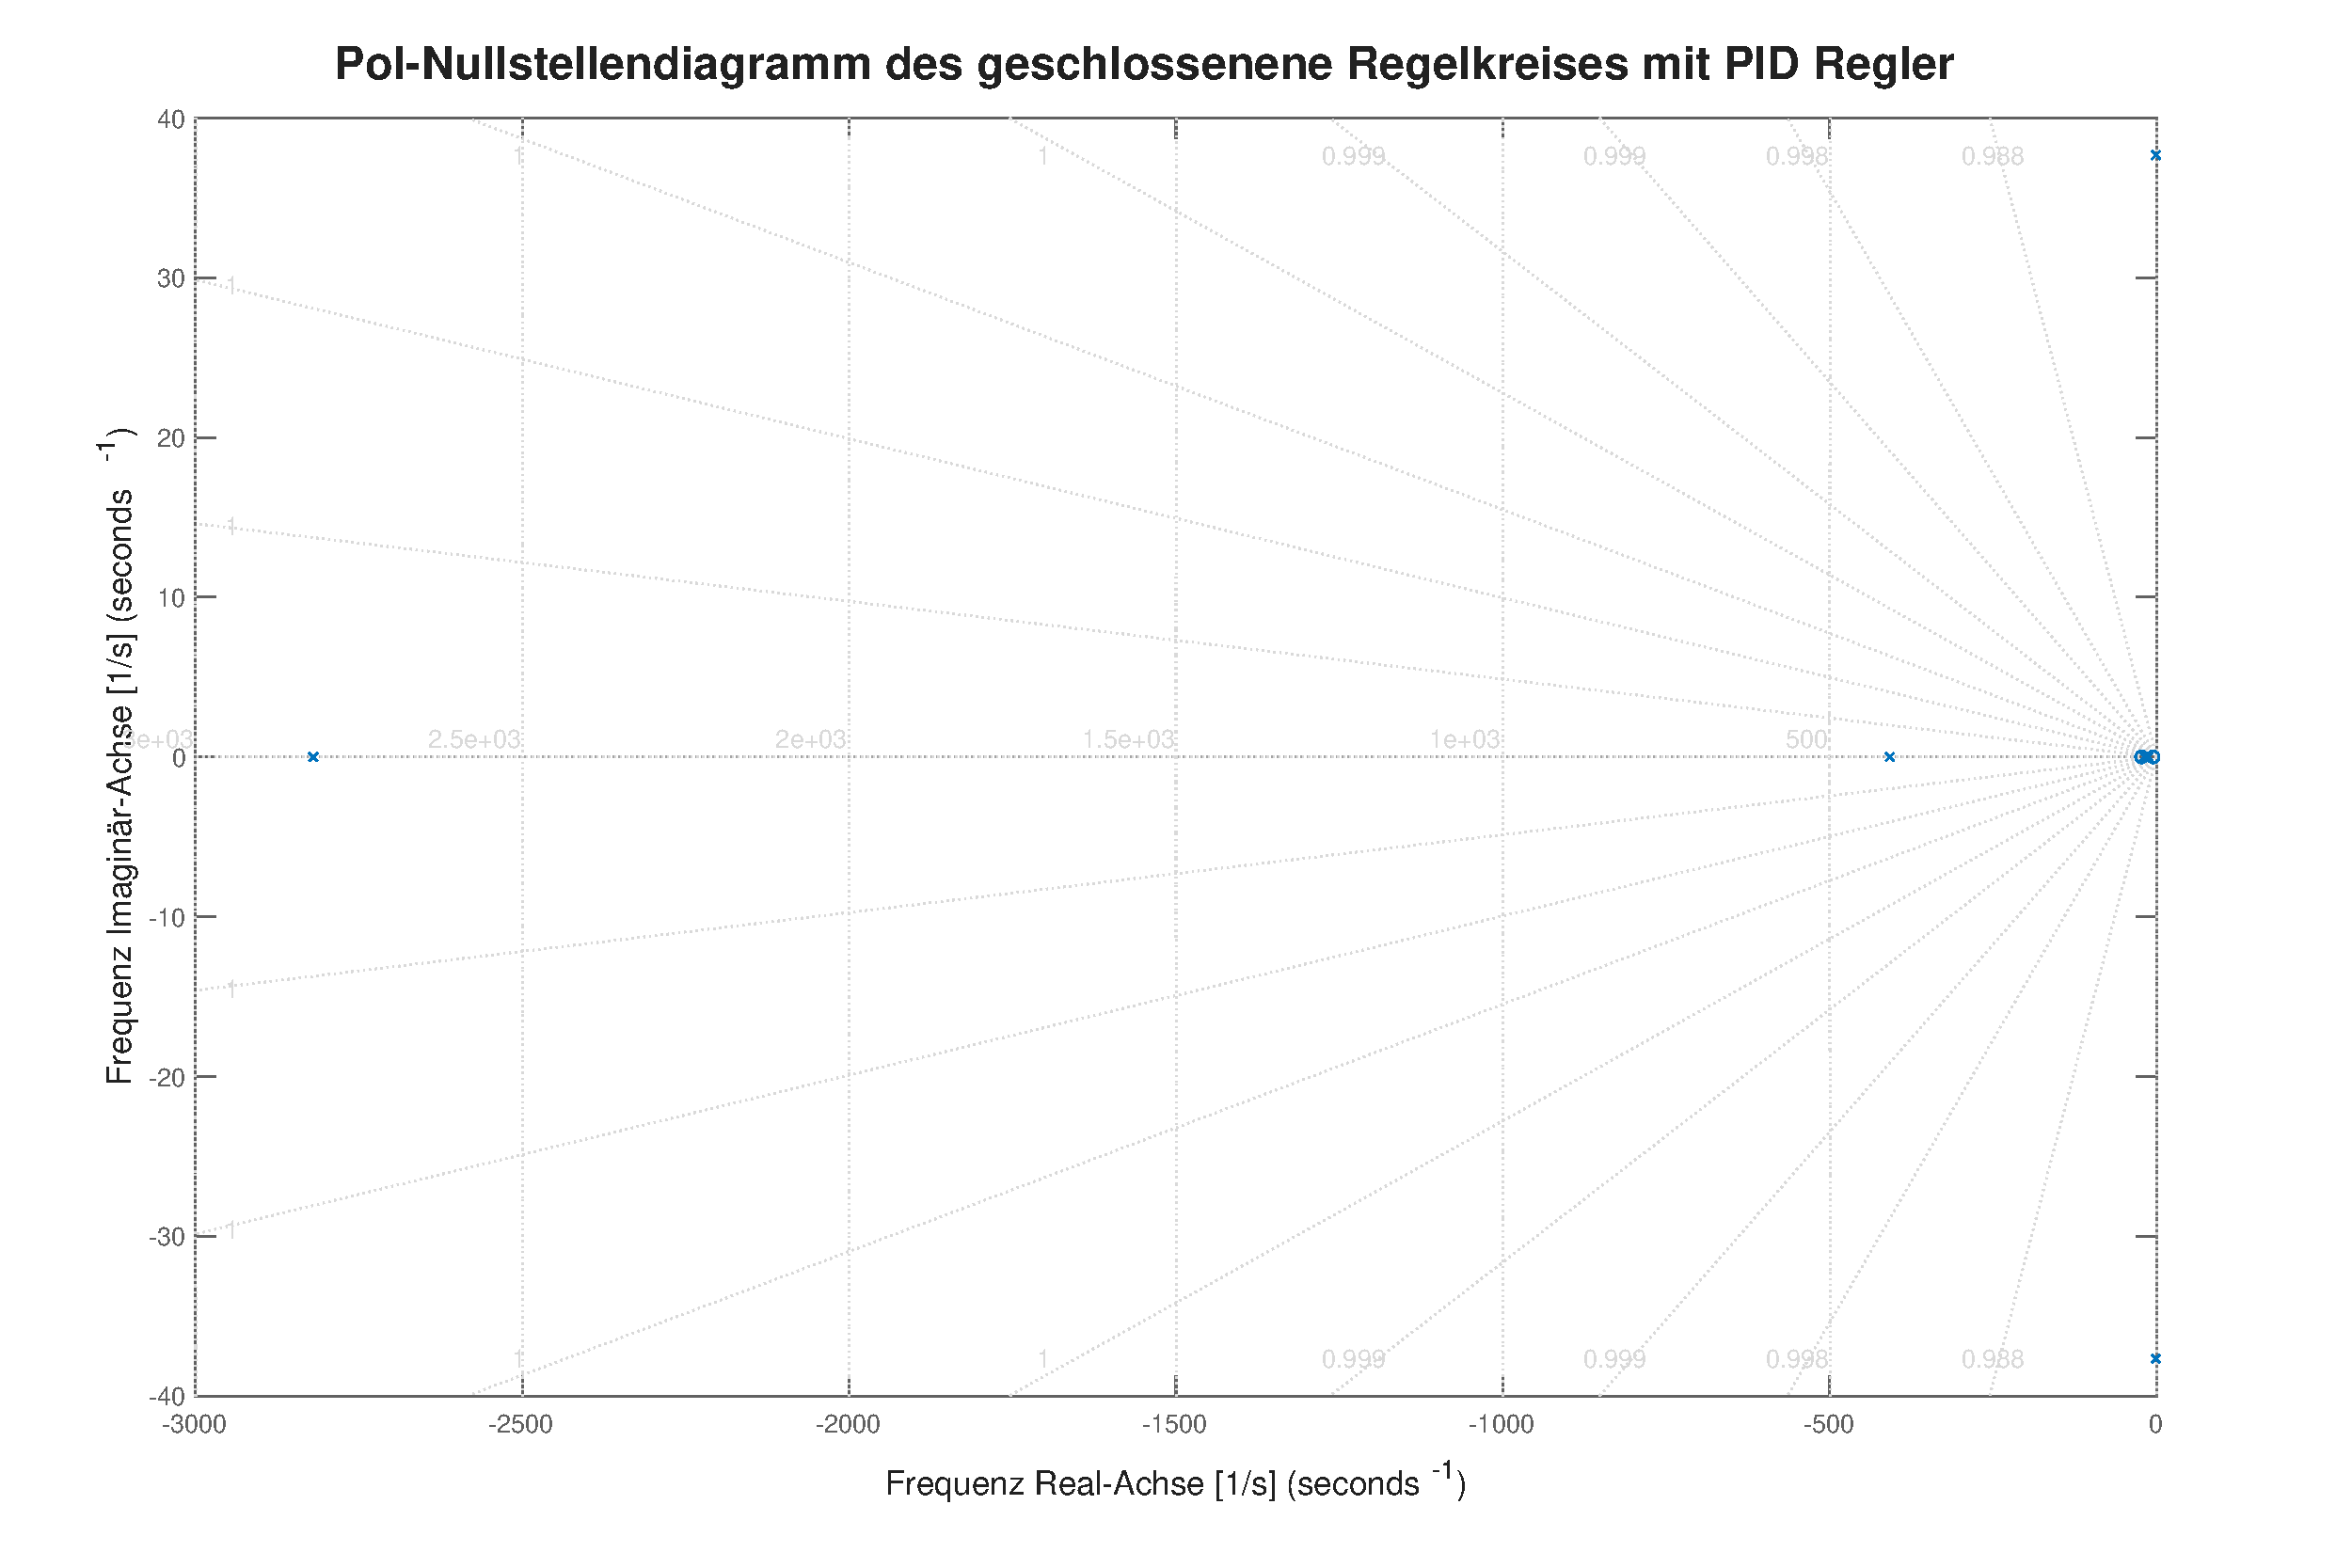
\includegraphics[width=.9\textwidth]{./figure/polemap_pid_untuned.pdf}
				\caption{Pole des Prozesses mit PID-Regler}
				\label{fig:polePID}
			\end{figure}


\newpage
\section{Aufgabe 16}\label{sec:Aufgabe16}
	\subsection*{Simulinkmodell des Aufbaus}
			\begin{figure}[H]
				\centering
				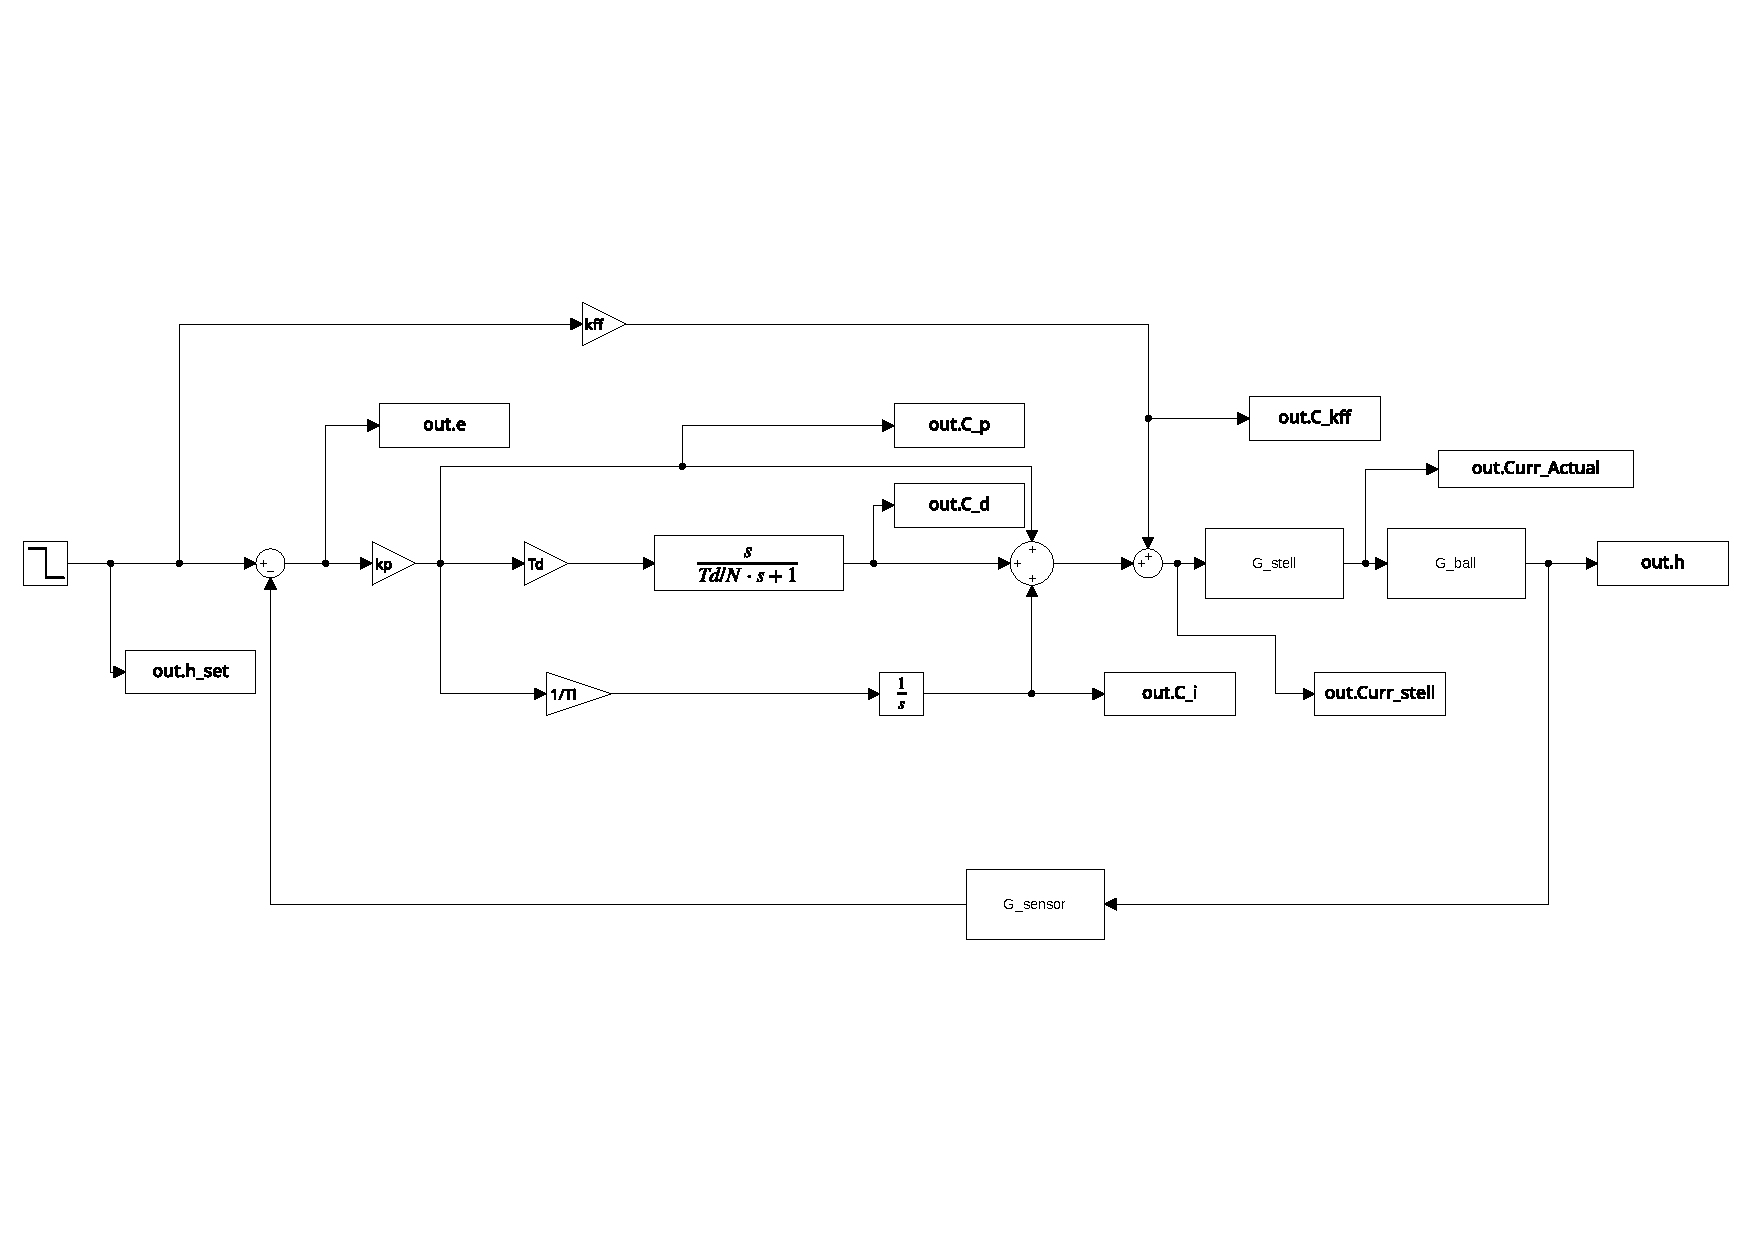
\includegraphics[width=\textwidth]{./figure/magnet_model.pdf}
				\caption{Simulink Modell inlusive Regler-, Stell-, Stecken- und Sensorübertrangungsfunktionen}
				\label{fig:model}
			\end{figure}
\newpage
\section{Aufgabe 17}\label{sec:Aufgabe17}
	\subsection*{Simulation Führungssprung}
	Zunächst wurde der PD-Regler mit einem Führungssprung von $x_0 = 40\si{\milli\meter}$ zu $x_1 = 35\si{\milli\meter}$ simuliert. In \autoref{fig:pd_simu} fällt dabei auf, dass der Regler zwar stabil scheint aber sich ein stationärer Fehler entsteht. Dieser Fehler ist ebenfalls weit von dem definierten Arbeitspunkt entfernt, womit der Regler möglicherweise am Versuch nicht funktionieren wird.
			\begin{figure}[H]
				\centering
				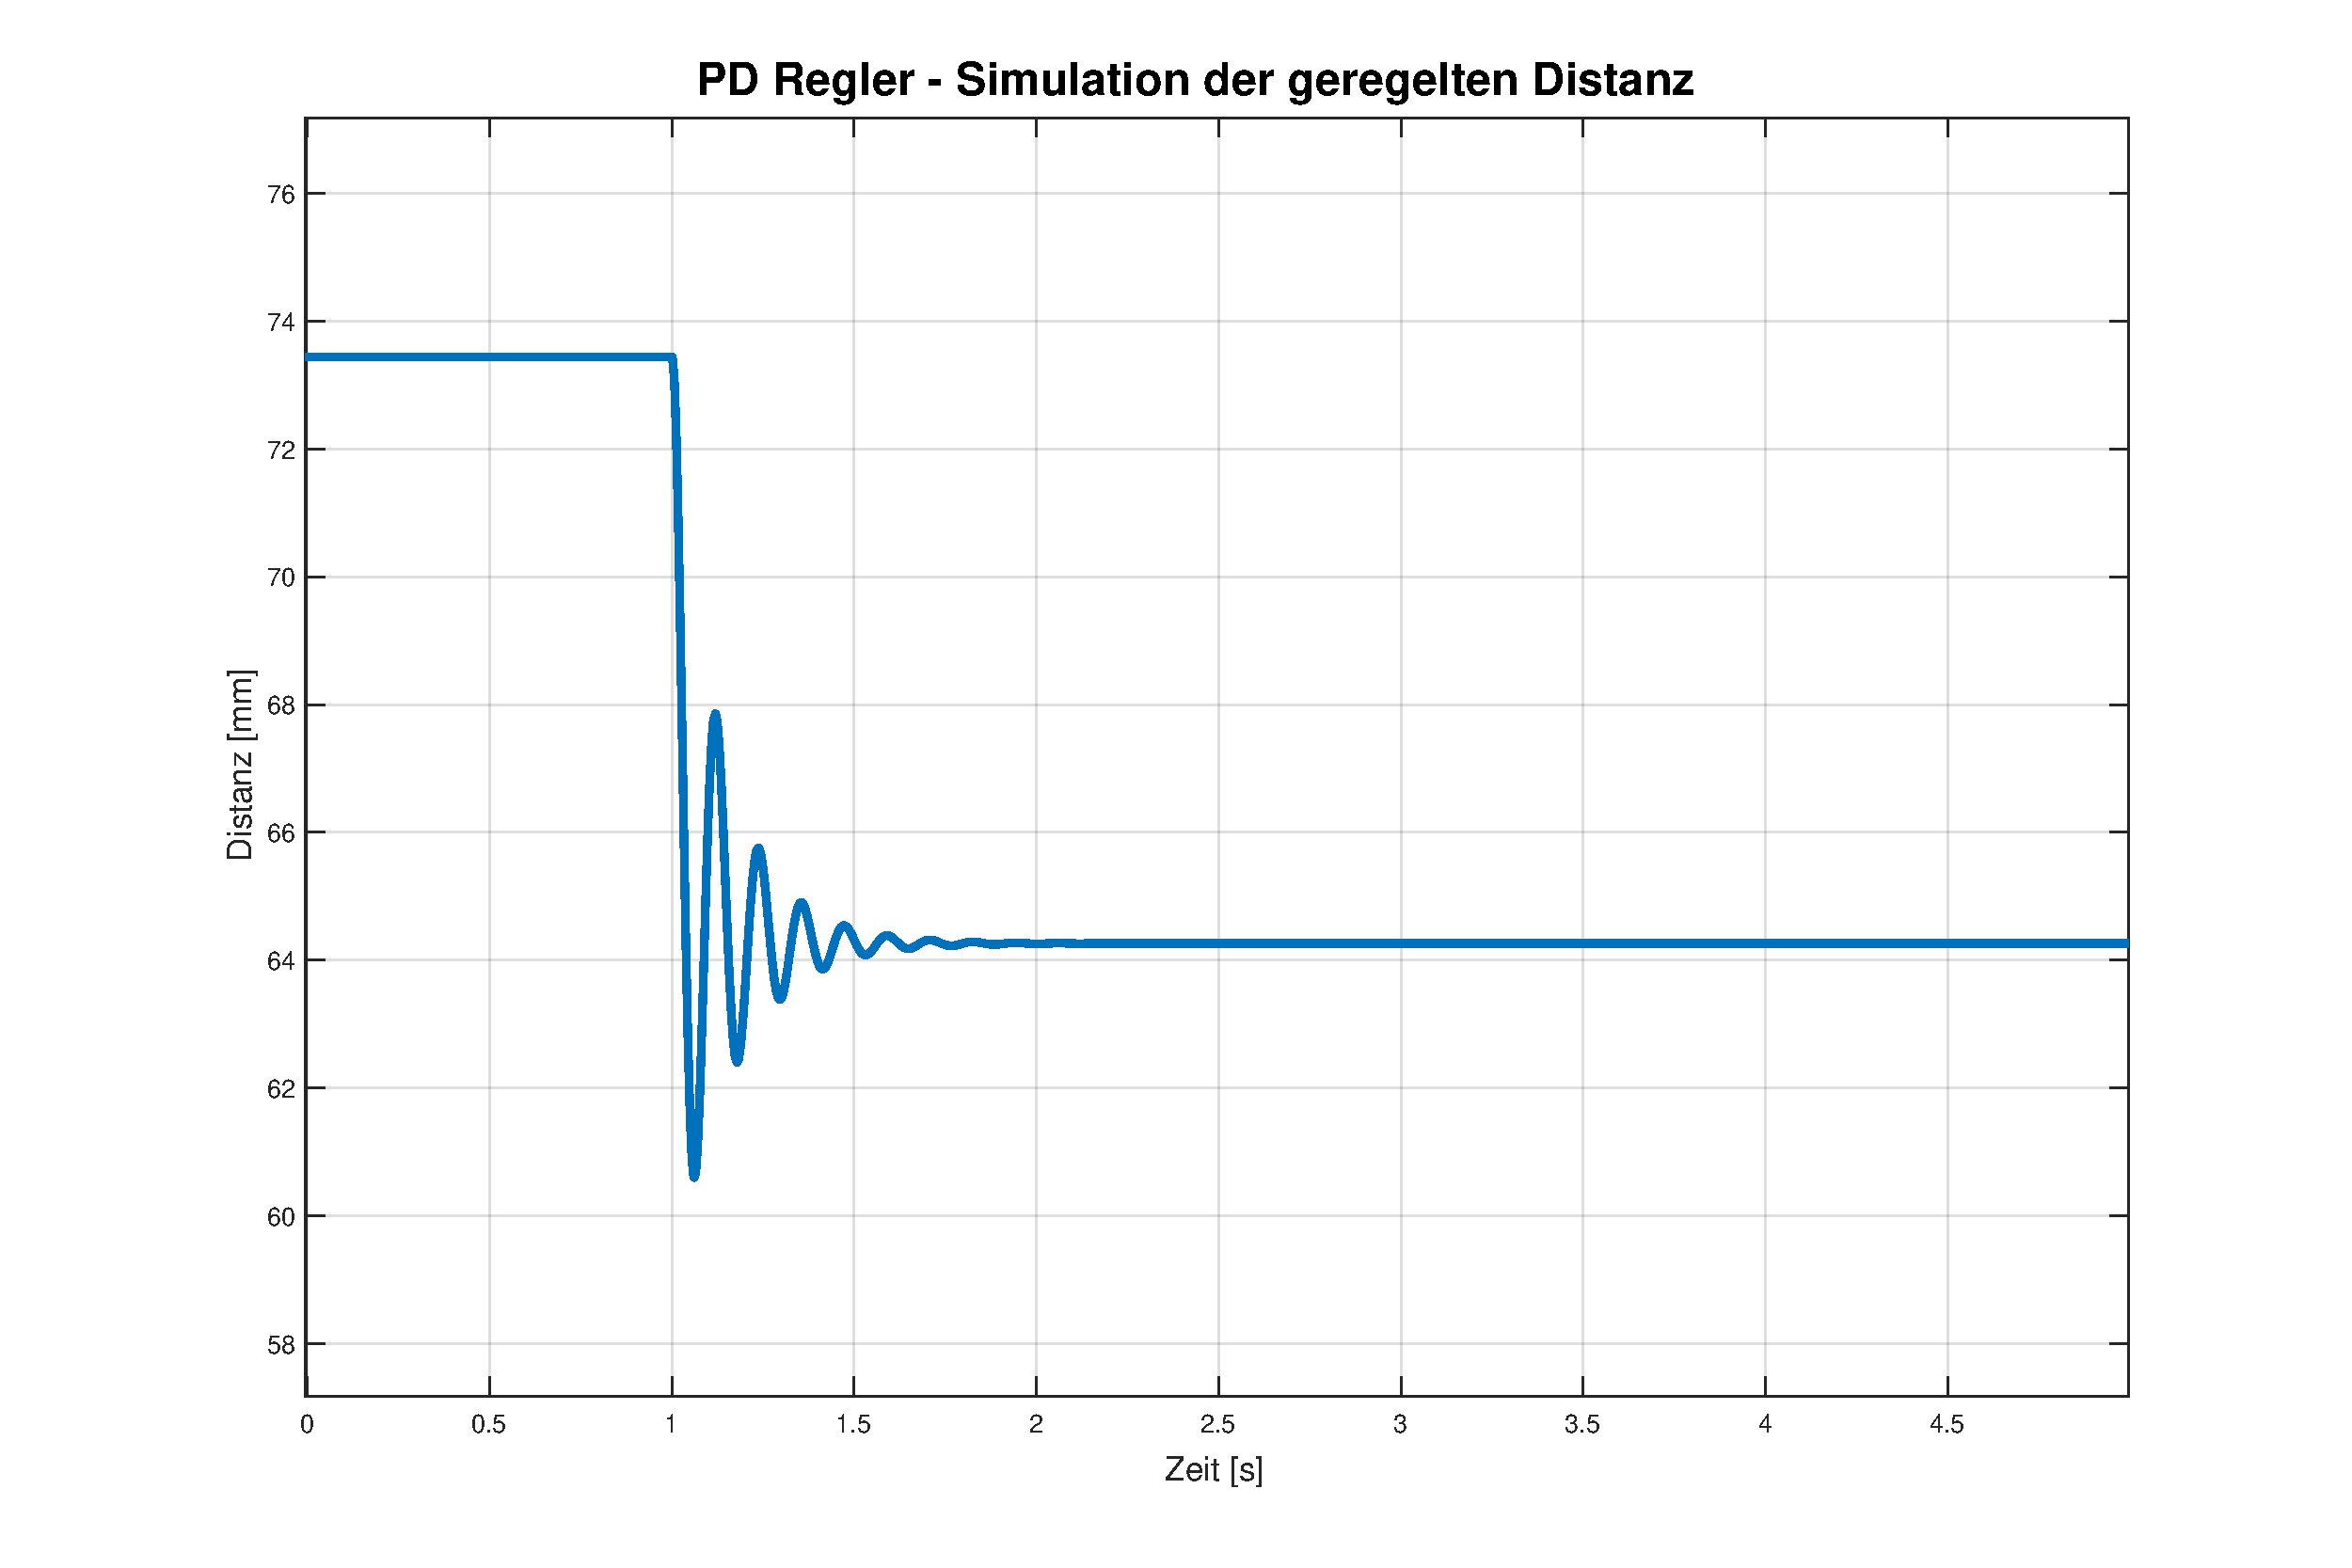
\includegraphics[width=\textwidth]{./figure/PD_simu.pdf}
				\caption{Simulierter Führungssprung mithilfe des PD-Reglers von $x_0 = 40\si{\milli\meter}$ zu $x_1 = 35\si{\milli\meter}$}
				\label{fig:pd_simu}
			\end{figure}


			Wird nun der PD-Regler auf einen PID-Regler erweitert, so stellt sich die gewünschten geregelten Distanzen von   $x_0 = 40\si{\milli\meter}$ zu $x_1 = 35\si{\milli\meter} $ korrekt ein, wie in \autoref{fig:pid_simu}	
			\begin{figure}[H]
				\centering
				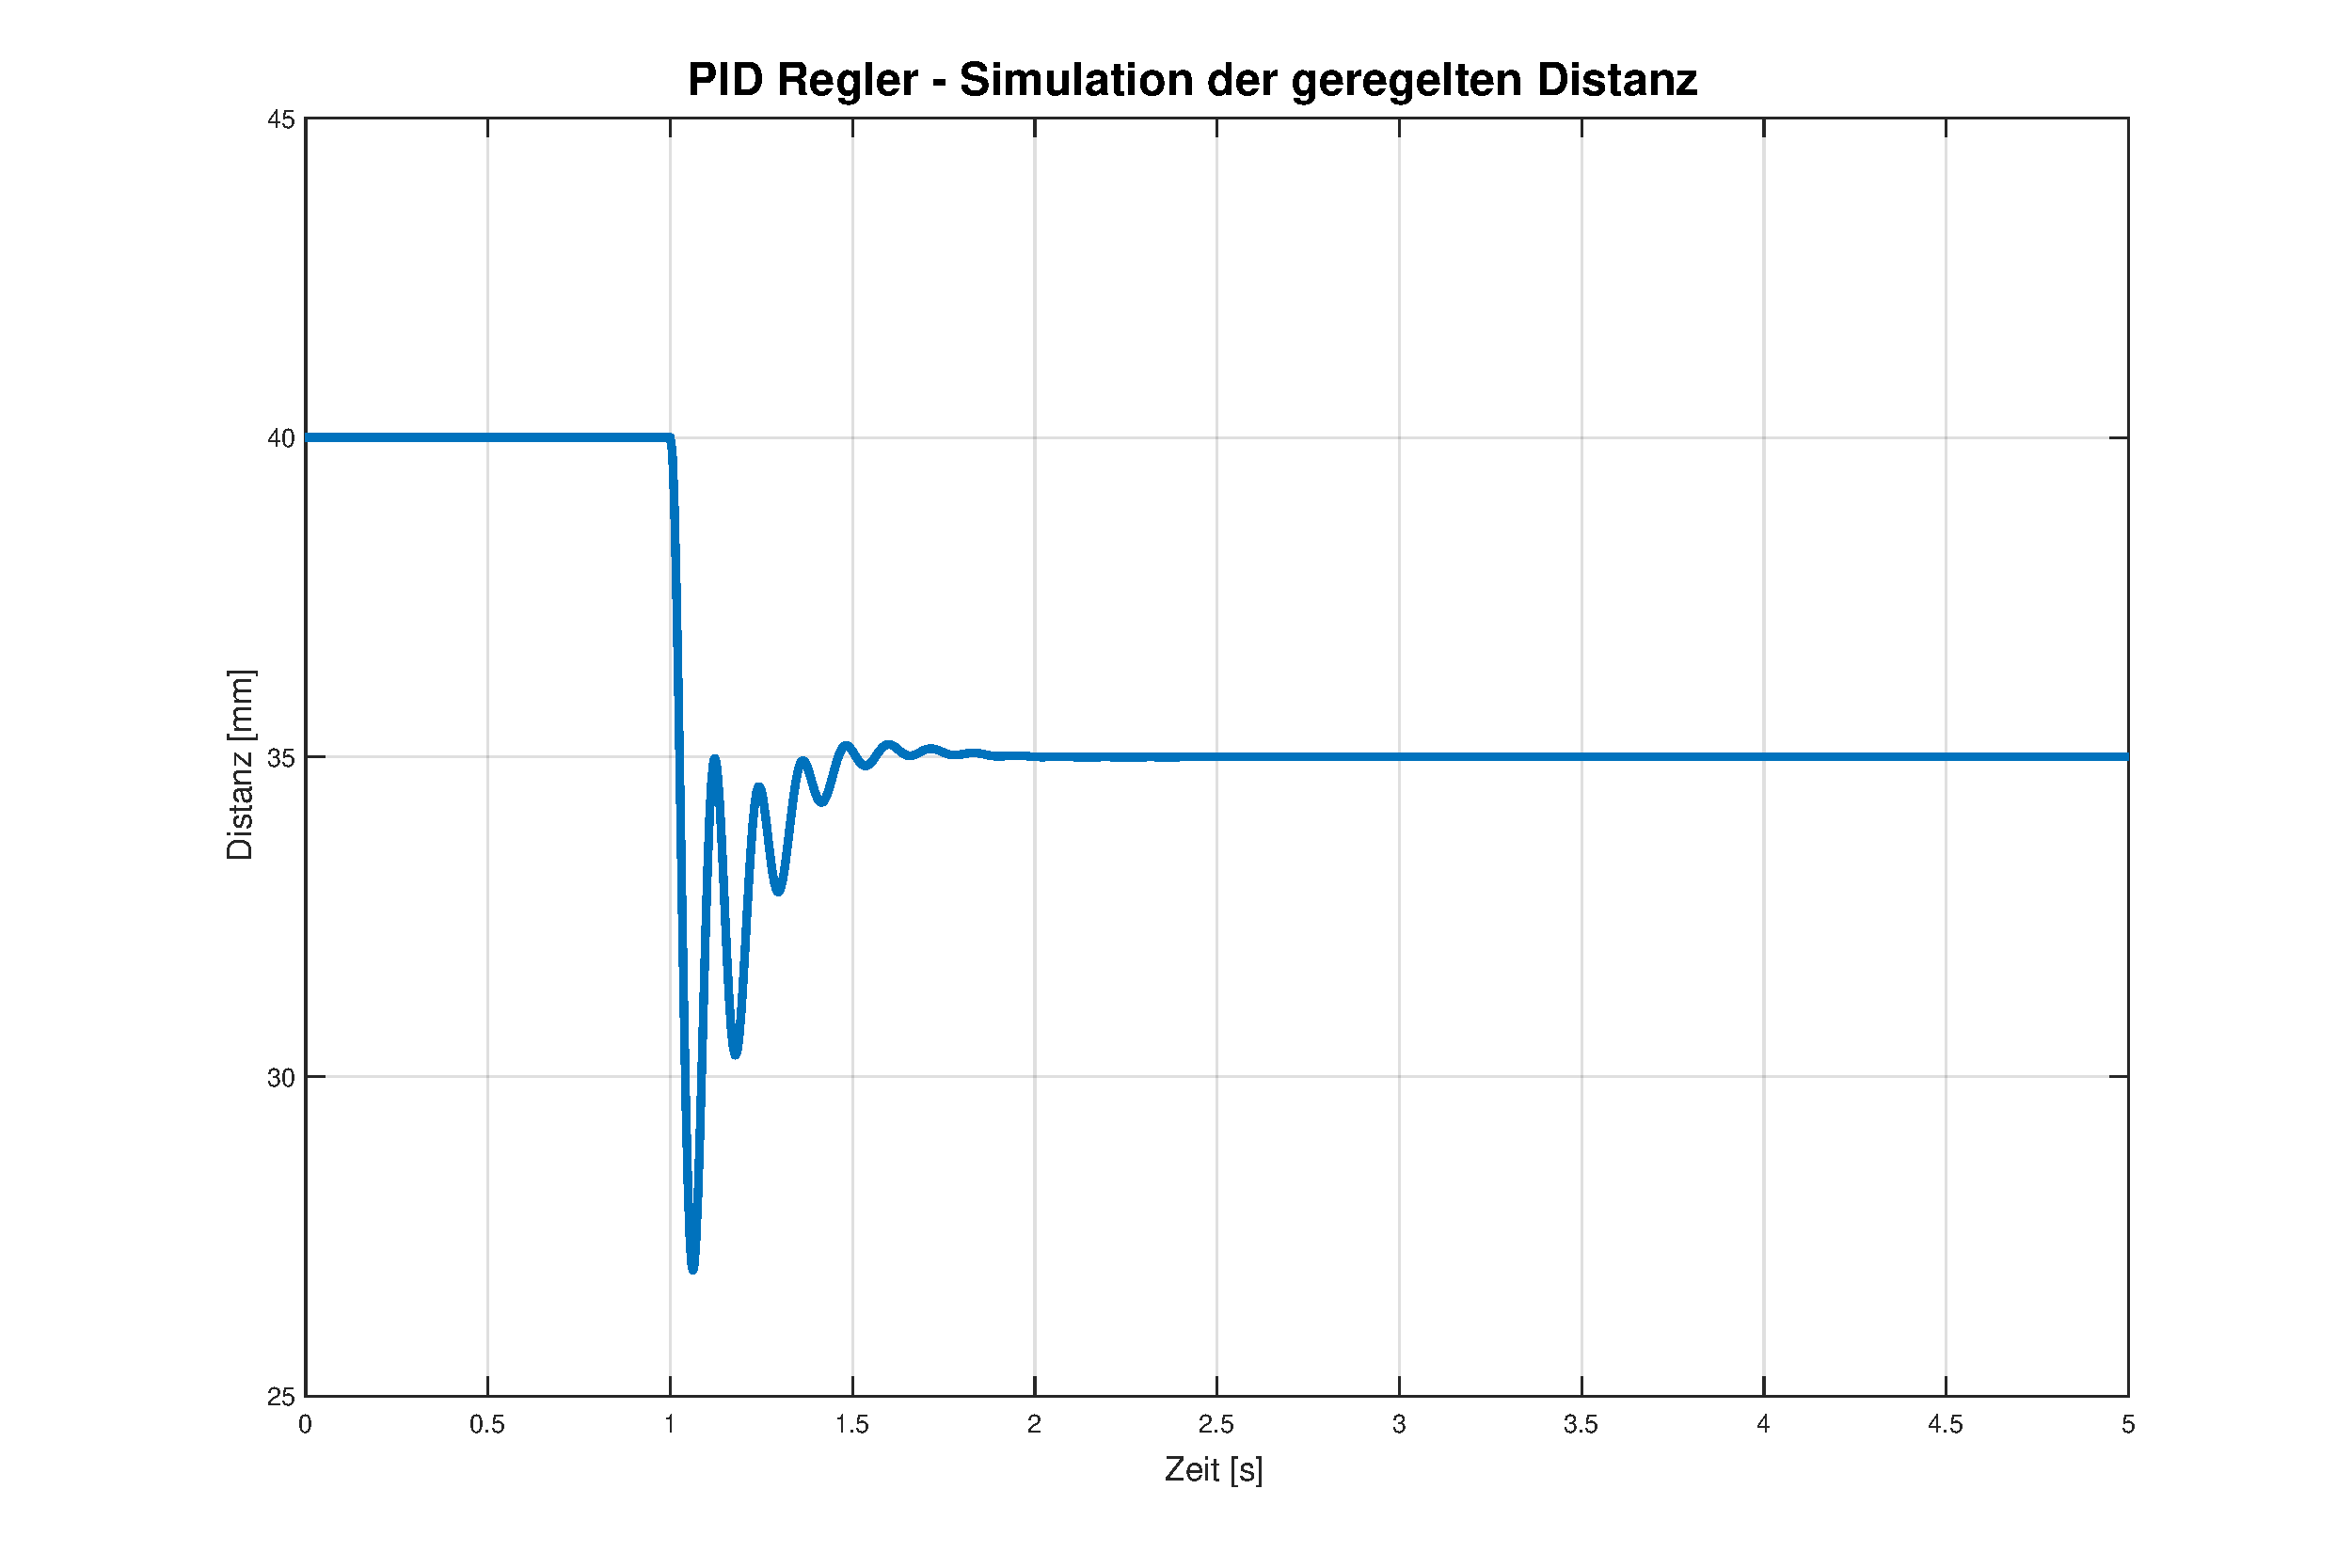
\includegraphics[width=\textwidth]{./figure/PID_simu.pdf}
				\caption{Simulierter Führungssprung mithilfe des PID-Reglers von $x_0 = 40\si{\milli\meter}$ zu $x_1 = 35\si{\milli\meter}$}
				\label{fig:pid_simu}
			\end{figure}
\newpage

\section{Aufgabe 18 und 19}\label{sec:Aufgabe1819}
	\subsection*{Verifikation am Versuch - PD}

	Der PD-Regler hat wie auch in der Simulation ersichtlich einen grossen stationären Fehler. Dies führt dazu, dass er bei $x_{ref}=40\si{\milli\meter}$ eine Distanz von $x_{eff}=60\si{\milli\meter}$ einzunehmen versucht. Dies ist zu weit entfernt, und der Laboraufbau kann nicht genug Strom liefern um den Ball auf Position zu halten. Deshalb wurde der Ball bei $x_0 = 30\si{\milli\meter}$ geregelt, um den simulierten Fehler trotzem überprüfen zu können.
			
		\begin{figure}[H]
				\centering
				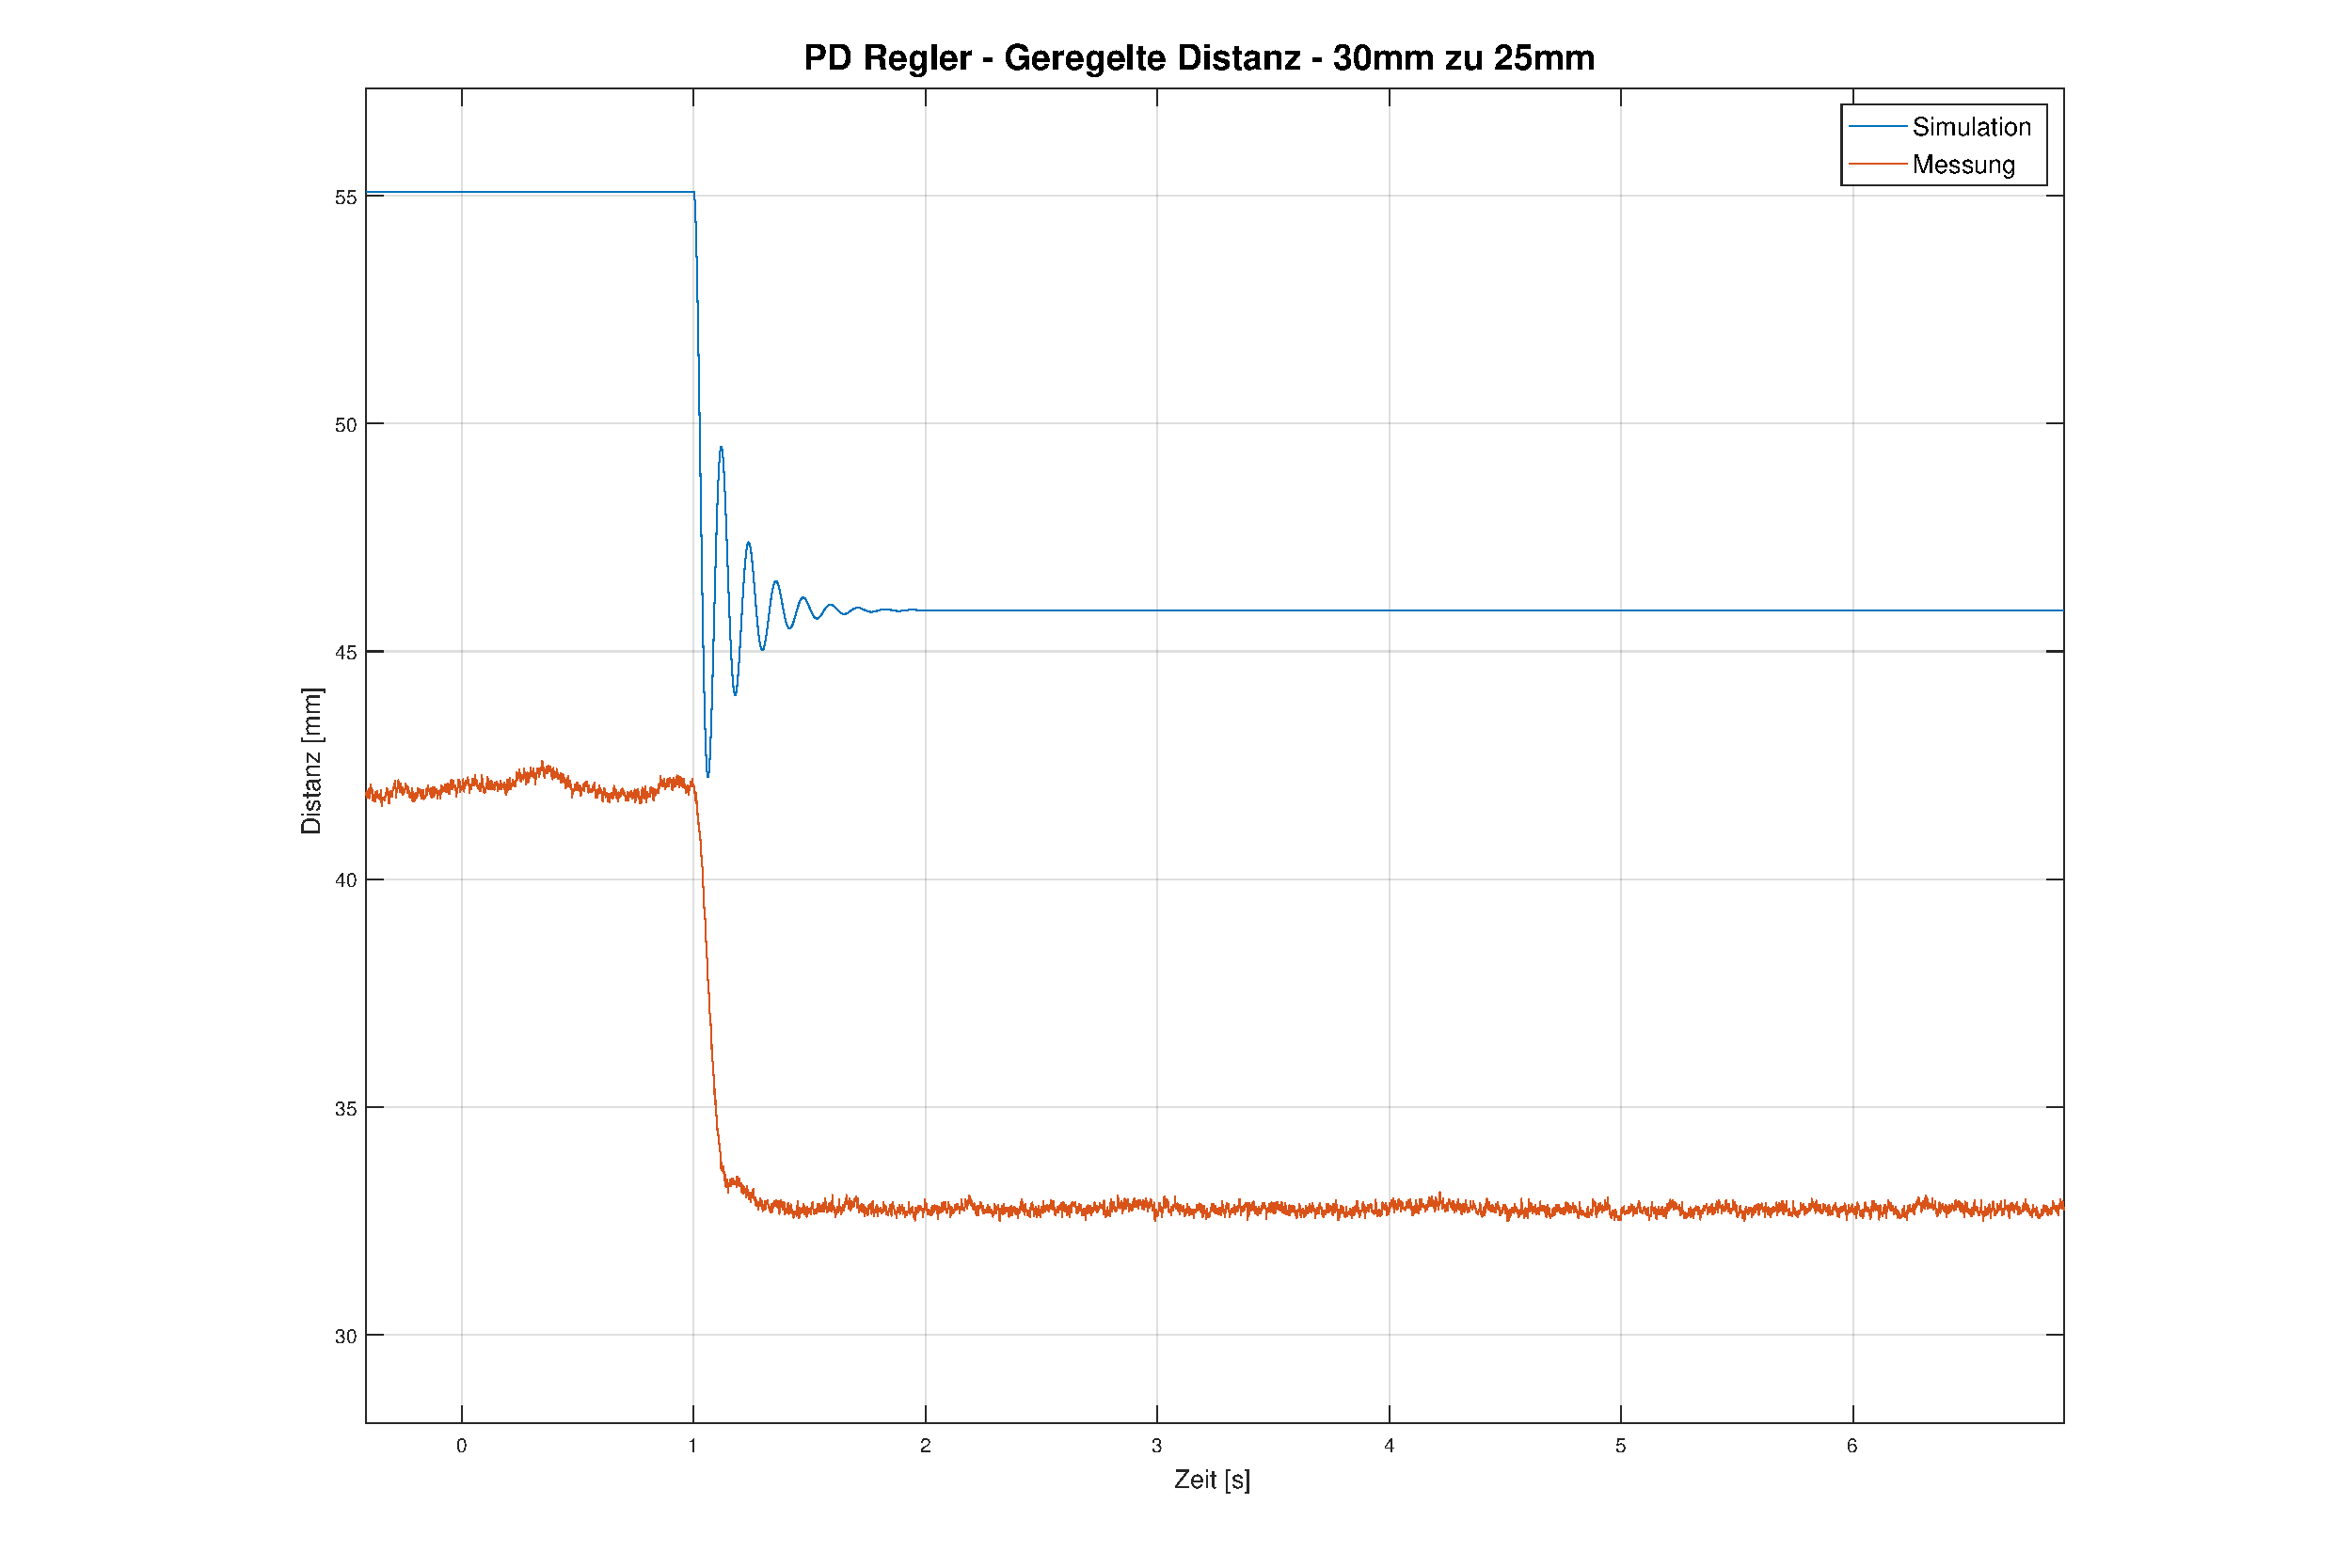
\includegraphics[width=\textwidth]{./figure/PD_mess_distanz.pdf}
				\caption{Simulierter und gemessener Führungssprung mithilfe des PD-Reglers von $x_0 = 30\si{\milli\meter}$ zu $x_1 = 25\si{\milli\meter}$}
				\label{fig:pd_mess}
			\end{figure}
			Hierbei wird in \autoref{fig:pd_mess} beobachtbar, dass laut Simulation der Regelfehler noch viel grösser wird, dies ist auf die weite Distanz zum Arbeitspunkt der Simulation zurückzuführen.

		\begin{figure}[H]
				\centering
				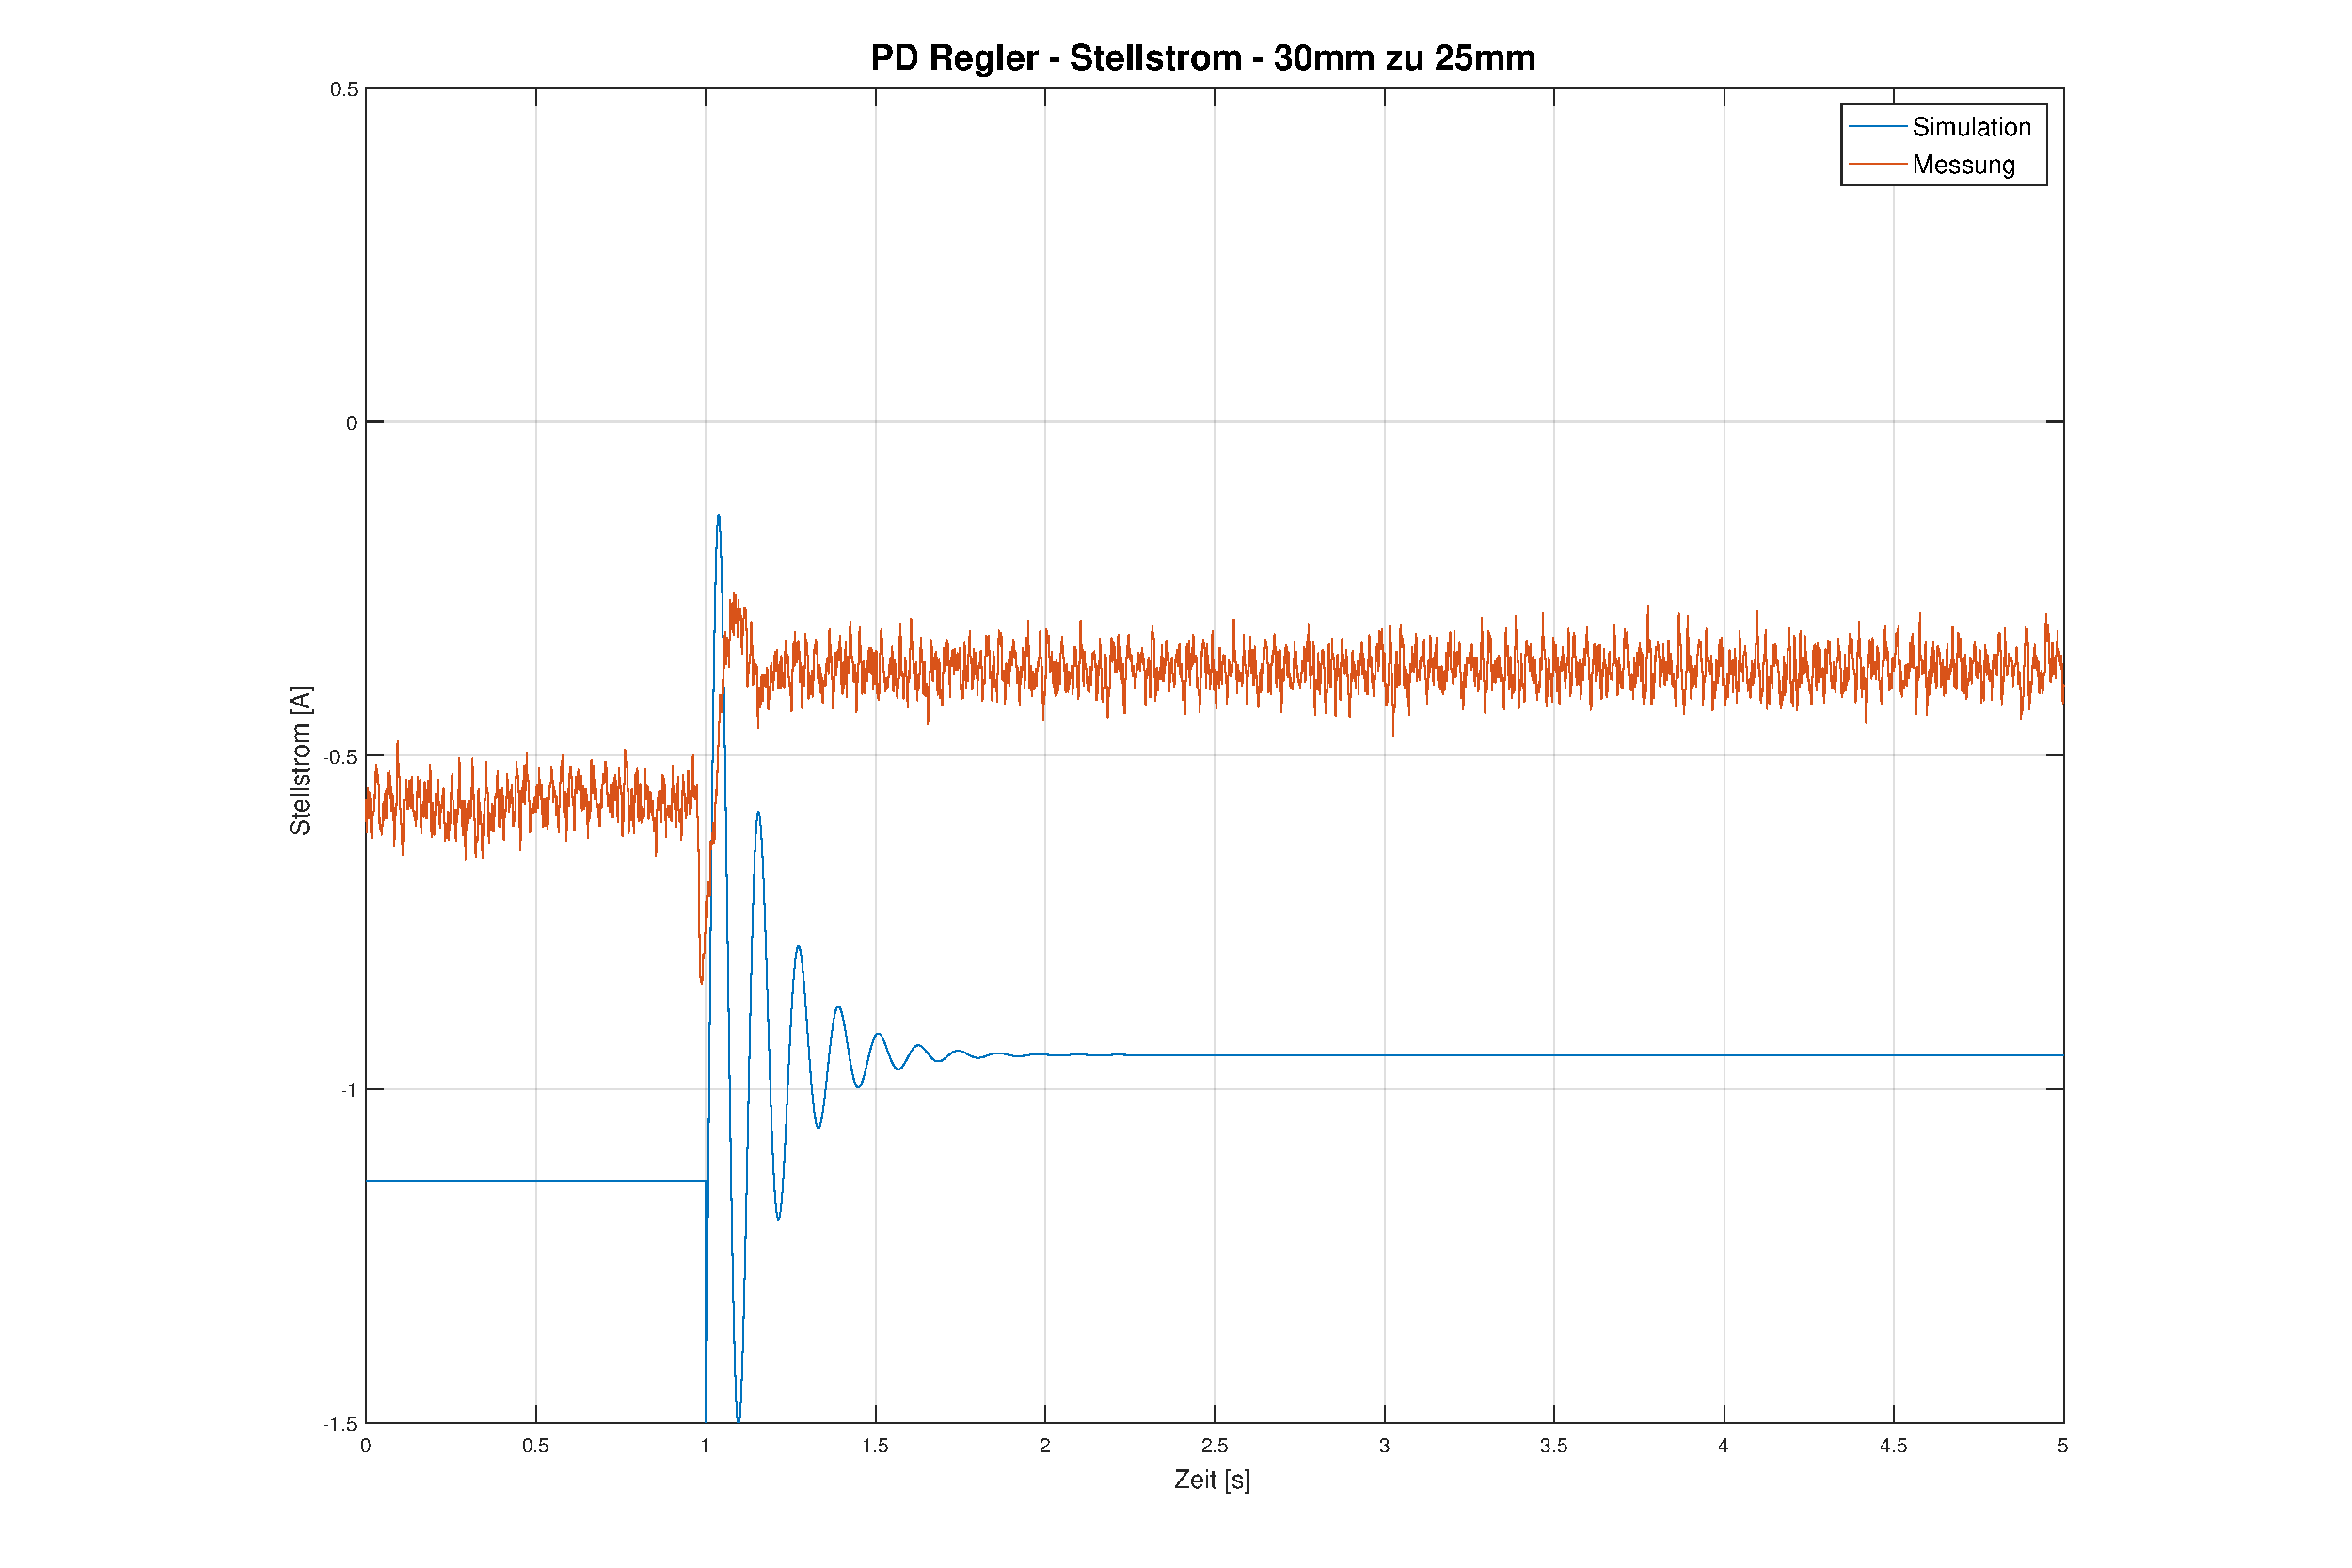
\includegraphics[width=\textwidth]{./figure/PD_mess_stellstrom.pdf}
				\caption{Simulierter und gemessener (SMA(20)) Stellstrom mithilfe des PD-Reglers von $x_0 = 30\si{\milli\meter}$ zu $x_1 = 25\si{\milli\meter}$}
				\label{fig:pd_mess_strom}
			\end{figure}


\newpage 
	\subsection*{Verifikation am Versuch - PID}
	Der PID-Regler hingegen regelt auf die korrekte Soll-Distanz von $x_0 = 40\si{\milli\meter}$ zu $x_1 = 35\si{\milli\meter}$. In \autoref{fig:pid_mess} ist der Vergleich zwischen Simulation und Messung ersichtlich. Erkennbar ist eine hohe Genauigkeit der Simulation bis auf ein nicht vorhandenes Einschwingen der Realität.
			
		\begin{figure}[H]
				\centering
				\includegraphics[width=\textwidth]{./figure/PiD_mess_distanz_40mm.pdf}
				\caption{Simulierter und gemessener Führungssprung mithilfe des PID-Reglers von $x_0 = 40\si{\milli\meter}$ zu $x_1 = 35\si{\milli\meter}$}
				\label{fig:pid_mess}
			\end{figure}
		Auch der Stellstrom in \autoref{fig:pid_mess_strom} ist plausiebler, wenn auch immernoch etwas von der Realität entfernt.
			\begin{figure}[H]
				\centering
				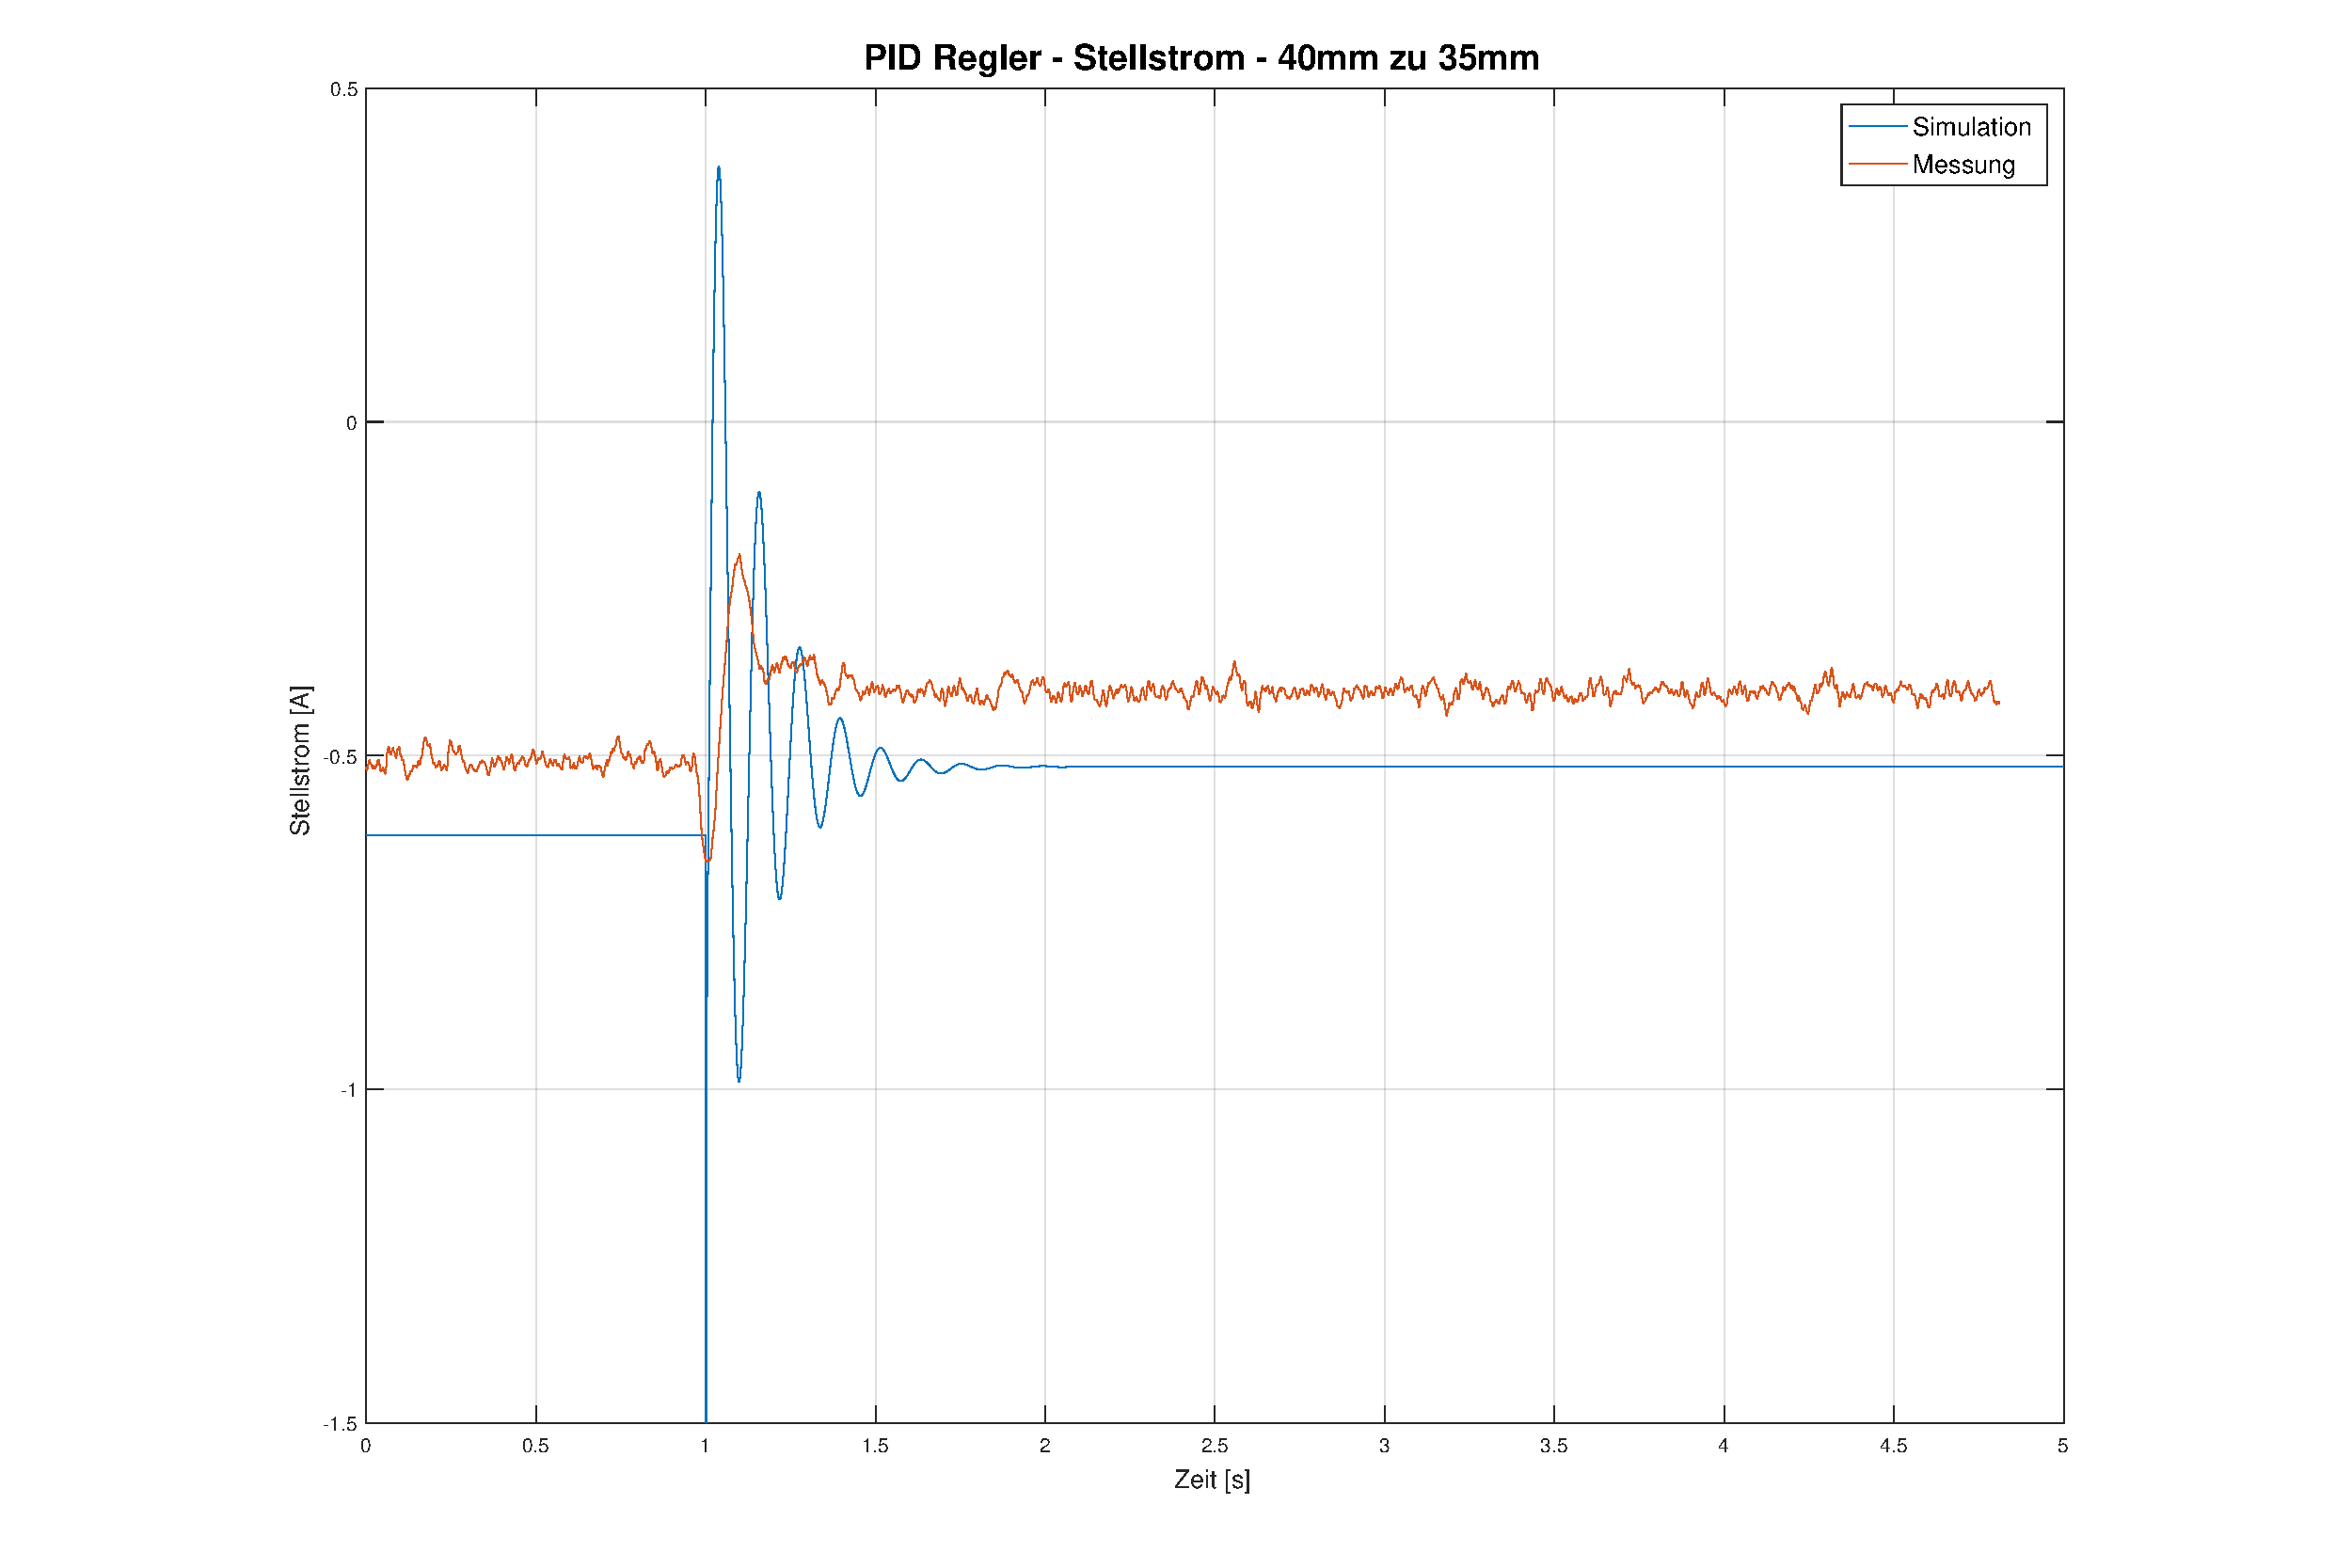
\includegraphics[width=\textwidth]{./figure/PID_mess_stellstrom_40mm.pdf}
				\caption{Simulierter und gemessener (SMA(20)) Stellstrom mithilfe des PID-Reglers von $x_0 = 30\si{\milli\meter}$ zu $x_1 = 25\si{\milli\meter}$}
				\label{fig:pid_mess_strom}
			\end{figure}


\section{Aufgabe 20}\label{sec:Aufgabe20}
	\subsection*{Verbesserung der Regler}
	Mittels Untersuchung der Wurzelortskurve und den Pollagen, wurde ein \textit{guter} PID-Regler entworfen mit den folgenden Paramerten:

		\begin{table}[!h]
			\renewcommand{\arraystretch}{1.2}
			\centering
			\caption{PID Regler Werte}
			\begin{zebratabular}{m{4cm} m{3cm}}
				\rowcolor{gray}
				\textbf{Parameter}	& \textbf{Wert} \\
				$k_p$				& $46$  \\ 
				$T_i$				& $0.3364$  \\
				$T_d$				& $0.0591$ \\
				$N$					& $100$ \\
			\end{zebratabular}
			\renewcommand{\arraystretch}{1.0}
			\label{tab:optimal}
		\end{table}


		\newpage

		Wie in \autoref{tab:optimal_pol} zu erkennen ist, wurden die kritischen Pole (also jene nahe an der Imaginärachse) weiter in den Imaginärteil verschoben, auf kosten der Pole die bereits weit entfernt waren die etwas näher rutschen.
		\begin{table}[!h]
			\renewcommand{\arraystretch}{1.2}
			\centering
			\caption{PID Regler Polunterschied}
			\begin{zebratabular}{m{2cm} m{5cm} m{5cm}}
				\rowcolor{gray}
				\textbf{Pol}	& \textbf{Ursprünglich} & \textbf{Verbessert}\\
				$P_1$				& $(-2.819)10^3$	&			$(-1.6911)10^3$\\
				$P_2$				& $(-0.4080)10^3$	&			$(-0.4138)10^3$\\
				$P_3$				& $(-0.0009 + 0.0377i)10^3$&	$(-0.0070 + 0.0527i)10^3$\\ 
				$P_4$				& $(-0.0009 - 0.0377i)10^3$& 	$(-0.0070 - 0.0527i)10^3$\\ 
				$P_5$				& $(-0.0180)10^3$	&			$(-0.0065 + 0.056i)10^3$\\ 
				$P_6$				& $(-0.0121)10^3$	&			$(-0.0065 - 0.056i)10^3$\\ 
			\end{zebratabular}
			\renewcommand{\arraystretch}{1.0}
			\label{tab:optimal_pol}
		\end{table}


\newpage

\section{Aufgabe 21}\label{sec:Aufgabe21}
	\subsection*{Pole ausserhalb des Arbeitspunkts}
	Wird nun der Arbeitspunkt weit weg vom Linearisierungspunkt gewählt wandern die Pole wiederum in die rechte Halbebene, was zu einem instabilen Prozess führt.
		\begin{table}[!h]
			\renewcommand{\arraystretch}{1.2}
			\centering
			\caption{Polpositionen bei verschiedenen Arbeitspunkten}
			\begin{zebratabular}{m{4.5cm} m{4.5cm} m{4.5cm}}
				\rowcolor{gray}
				$x_0 = 40\si{\milli\meter}$ &  $x_0 = 30\si{\milli\meter}$ & $x_0 = 50\si{\milli\meter}$\\
				$(-1.6911)10^3$								& $(-1.1678)10^3$	&				$(-1.6918)10^3$\\
				$(-0.4138)10^3$								& $(-0.4647)10^3$	&				$(-0.4046)10^3$\\
				$(-0.0070 + 0.0527i)10^3$					& $(0.0160 + 0.1.235i)10^3$&		$(-0.0320 + 0.0215i)10^3$\\ 
				$(-0.0070 - 0.0527i)10^3$					& $(0.0160 - 0.1235i)10^3$&			$(-0.0320 - 0.0215i)10^3$\\ 
				$(-0.0065 + 0.056i)10^3$					& $(-0.0057 + 0.0057i)10^3$	&		$(0.0269)10^3$\\ 
				$(-0.0065 - 0.056i)10^3$					& $(-0.0057 - 0.0057i)10^3$	&		$(0.0016)10^3$\\ 
			\end{zebratabular}
			\renewcommand{\arraystretch}{1.0}
			\label{tab:optimal_pol}
		\end{table}




\end{document}
